% Format teze zasnovan je na paketu memoir
% http://tug.ctan.org/macros/latex/contrib/memoir/memman.pdf ili
% http://texdoc.net/texmf-dist/doc/latex/memoir/memman.pdf
% 
% Prilikom zadavanja klase memoir, navedenim opcijama se podešava 
% veličina slova (12pt) i jednostrano štampanje (oneside).
% Ove parametre možete menjati samo ako pravite nezvanične verzije
% mastera za privatnu upotrebu (na primer, u b5 varijanti ima smisla 
% smanjiti 
\documentclass[12pt,oneside]{memoir}

% Paket koji definiše sve specifičnosti mastera Matematičkog fakulteta
\usepackage{matfmaster}
%
% Podrazumevano pismo je ćirilica.
%   Ako koristite pdflatex, a ne xetex, sav latinički tekst na srpskom jeziku
%   treba biti okružen sa \lat{...} ili \begin{latinica}...\end{latinica}.
%
% Opicija [latinica]:
%   ako želite da pišete latiniciom, dodajte opciju "latinica" tj.
%   prethodni paket uključite pomoću: \usepackage[latinica]{matfmaster}.
%   Ako koristite pdflatex, a ne xetex, sav ćirilički tekst treba biti
%   okružen sa \cir{...} ili \begin{cirilica}...\end{cirilica}.
%
% Opcija [biblatex]:
%   ako želite da koristite reference na više jezika i umesto paketa
%   bibtex da koristite BibLaTeX/Biber, dodajte opciju "biblatex" tj.
%   prethodni paket uključite pomoću: \usepackage[biblatex]{matfmaster}
%
% Opcija [b5paper]:
%   ako želite da napravite verziju teze u manjem (b5) formatu, navedite
%   opciju "b5paper", tj. prethodni paket uključite pomoću: 
%   \usepackage[b5paper]{matfmaster}. Tada ima smisla razmisliti o promeni
%   veličine slova (izmenom opcije 12pt na 11pt u \documentclass{memoir}).
%
% Naravno, opcije je moguće kombinovati.
% Npr. \usepackage[b5paper,biblatex]{matfmaster}

% Pomoćni paket koji generiše nasumičan tekst u kojem se javljaju sva slova
% azbuke (nema potrebe koristiti ovo u pravim disertacijama)
\usepackage{pangrami}

% Paket koji obezbeđuje ispravni prikaz ćiriličkih italik slova kada
% se koristi pdflatex. Zakomentarisati ako na sistemu koji koristite ovaj
% paket nije dostupan ili ako ne radi ispravno.
\usepackage{cmsrb}

% Ostali paketi koji se koriste u dokumentu
\usepackage{listings} % listing programskog koda

\renewcommand\lstlistingname{К\^{о}д}
\renewcommand\lstlistlistingname{К\^{о}д}

\usepackage{xcolor}

\definecolor{codegreen}{rgb}{0,0.6,0}
\definecolor{codegray}{rgb}{0.5,0.5,0.5}
\definecolor{codepurple}{rgb}{0.58,0,0.82}
\definecolor{backcolour}{rgb}{0.94,0.94,0.94}

\lstdefinestyle{mystyle}{
    basicstyle=\sffamily,
    backgroundcolor=\color{backcolour},   
    commentstyle=\color{codegreen},
    keywordstyle=\color{red},
    numberstyle=\tiny\color{codegray},
    stringstyle=\color{codepurple},
    breakatwhitespace=false,         
    breaklines=true,                 
    captionpos=b,                    
    keepspaces=true,                 
    %numbers=left,                    
    numbersep=5pt,                  
    showspaces=false,                
    showstringspaces=false,
    showtabs=false,                  
    tabsize=2
}

\lstset{style=mystyle}

% Datoteka sa literaturom u BibTex tj. BibLaTeX/Biber formatu
\bib{matfmaster-primer}

% Ime kandidata na srpskom jeziku (u odabranom pismu)
\autor{Давид Гавриловић}
% Naslov teze na srpskom jeziku (u odabranom pismu)
\naslov{Дистрибуирана обрада геопросторних података}
% Godina u kojoj je teza predana komisiji
\godina{2022}
% Ime i afilijacija mentora (u odabranom pismu)
\mentor{др Мика \textsc{Микић}, редован професор\\ Универзитет у Београду, Математички факултет}
% Ime i afilijacija prvog člana komisije (u odabranom pismu)
\komisijaA{др Ана \textsc{Анић}, ванредни професор\\ University of Disneyland, Недођија}
% Ime i afilijacija drugog člana komisije (u odabranom pismu)
\komisijaB{др Лаза \textsc{Лазић}, доцент\\ Универзитет у Београду, Математички факултет}
% Ime i afilijacija trećeg člana komisije (opciono)
% \komisijaC{}
% Ime i afilijacija četvrtog člana komisije (opciono)
% \komisijaD{}
% Datum odbrane (obrisati ili iskomentarisati narednu liniju ako datum odbrane nije poznat)
\datumodbrane{15. јануар 2016.}

% Apstrakt na srpskom jeziku (u odabranom pismu)
\apstr{%
\pangrami
}

% Ključne reči na srpskom jeziku (u odabranom pismu)
\kljucnereci{анализа, геометрија, алгебра, логика, рачунарство, астрономија}

\begin{document}
% ==============================================================================
% Uvodni deo teze
\frontmatter
% ==============================================================================
% Naslovna strana
\naslovna
% Strana sa podacima o mentoru i članovima komisije
\komisija
% Strana sa posvetom (u odabranom pismu)
\posveta{некоме}
% Strana sa podacima o disertaciji na srpskom jeziku
\apstrakt
% Sadržaj teze
\tableofcontents*

% ==============================================================================
% Glavni deo teze
\mainmatter
% ==============================================================================


\chapter{Увод}
\label{chp:uvod}

увод о свему у раду

\textbf{TODO}

\chapter{Програмски језик Скала}
\label{chp:scala}

Скала (енг. Scala) је виши програмски језик заснован на функционалној и објектно оријентисаној парадигми. Име је добила од енглеске речи \textit{scalable} јер је дизајнирана тако да се развија са потребама корисника. Има широк спектар примена и може се користити за писање једноставних скрипти али и у изградњи великих и комплексних система. \cite{scala_prog}

Настала је 2001. на швајцарском федералном институту за технологију у Лозани (фра. \textit{École Polytechnique Fédérale de Lausanne}) и њен творац је Мартин Одерски (енг. \textit{Martin Odersky}). Прва званична верзија је изашла 20. јануара 2004. године.

Данас је широко распрострањена и користе је велике корпорације, као што су \textit{Twitter}, \textit{Google} и \textit{Apple}. Поред тога, веома је заступљена у заједници отвореног кода у пројектима као што су \textit{Apache Spark}, \textit{Apache Kafka}, \textit{Apache Flink} и \textit{Akka}.

\section{Особине језика \textit{Scala}}
\label{sec:osоб_scala}

\textit{Scala} је спој две парадигме, објектно оријентисане и функционалне, па стога поседује велики број особина. Поред тога, компајлира се на исти начин као и језик Јава, са којим постоје одређене сличности.

\subsection{Објектно оријентисан и функционалан језик}
\label{subsec:scala_obj_prog}

Скала је у потпуности објектно оријентисан језик. То значи да је свака вредност која се дефинише објекат, као и да је свака акција која се позива метод. На пример, уколико се врши одузимање два цела броја, позива се метод назван $''-''$ (минус). Тај метод је дефинисан у класи која представља целе бројеве, \textit{Int}. \cite{scala_prog}

Поред тога што је објектно оријентисан језик, \textit{Scala} је и функционалан језик. Функционално програмирање је засновано на два принципа. Први је да су функције вредности првог реда. То значи да се функције посматрају на исти начин као и други типови, на пример целобројни или ниска. Такође, функције је могуће прослеђивати другим функцијама, функције могу бити повратна вредност неке друге функције и функције се могу складиштити у променљивама.

Други принцип је да функције које се позивају немају бочне ефекте. Једна функција има улогу само да пресликава улаз у одговарајући излаз. То значи да ће сваки позив једне функције са истом вредношћу улазних аргумената, увек резултовати истом излазном вредношћу, независно од тога када се функција позива током извршавања програма. Другачији назив за ову особину је транспарентост референци. \cite{scala_prog}

Из овога произилази да функционални језици користе имутабилне структуре података. То су такве структуре за које важи да се подаци унутар њих не мењају. Уколико до промене мора доћи, сама структура се не мења, већ се од ње конструише тотално нова, са измењеним вредностима. \cite{scala_prog}

Међутим, Скала није чисто функционалан језик, што значи да се ипак може дефинисати функција која поседује бочне ефекте или се могу користити структуре података које се могу мењати. Поред тога, Скала омогућава писање функционалног кода без бочних ефеката и са имутабилним структурама података, па се може користити и на тај начин. \cite{scala_prog}

\subsection{Повезаност са језиком Јава}
\label{subsec:scala_komp}

\textit{Scala} је конструисана тако да се компајлира у Јавин ЈВМ бајтк\^{о}д (енг. \textit{Java JVM bytecode}). То значи да \textit{Scala} може користити Јава класе, методе и типове. На пример, Скалин објектни целобројни тип у својој имплементацији користи примитивни еквивалент из Јаве. Поред тога, Скала може користити Јава к\^{о}д и обогатити га на неки начин, као на пример додавањем неке методе у већ постојећу класу. Напоменимо и то да је време извршавања Скала програма приближно извршавању Јава програмима. \cite{scala_prog}

Међутим, иако се компајлирају на исти начин, програми написани у језику Скала често садрже мањи број линија од оних написаних у језику Јава. У неким случајевима се очекује да је к\^{о}д чак дупло краћи. Краћи програми доводе до тога да је к\^{о}д лакше писати и разумети, али и до мање вероватноће прављења грешака. \cite{scala_prog}

Један од многих примера како Скала смањује број линија у односу на Јаву је приказан у кодовима \ref{lst:scala_java_class_declaration} и \ref{lst:scala_scala_class_declaration} који представљају начине декларисања класе у та два програмска језика.

\begin{lstlisting}[caption={Декларација класе у језику Јава}, language=Java, label={lst:scala_java_class_declaration}]
// Java
class MyClass {  
  private int index;
  private String name;
  
  public MyClass(int index, String name) {
    this.index = index;
    this.name = name;
  }
}
\end{lstlisting}

\begin{lstlisting}[caption={Декларација класе у језику Scala}, language=Scala, label={lst:scala_scala_class_declaration}]
// Scala
class MyClass(index: Int, name: String)

\end{lstlisting}

У Скали се не мора декларисати посебна конструктор фукција, што доводи до смањења броја линија кода. \cite{scala_prog}

\subsection{Статичка типизираност}
\label{subsec:scala_stat_tip}

Статичка типизираност значи да се типови променљивих закључују за време компилације програма. То је супротно од динамичке типизираности која то чини за време извршавања. Оба приступа имају своје предности и мане. Скала је статички типизиран језик и поседује веома напредан систем типова.

То доноси предности које доводе до лакшег откривања грешака приликом писања кода. На пример, у статички типизираним програмима се током компилације сазнаје да ли је примењена нека операција на тип над којим та операција није дозвољена. Поред тога, статичка типизираност чини рефакторисање кода поузданијим. На пример, након измене метода се са сигурношћу може рећи да се повратни тип није променио. \cite{scala_prog}

Скала није само статички типизиран језик већ је и језик који аутоматски закључује типове у току компилације. На пример, када се декларише нека променљива целобројног типа, нема потребе назначити и њен тип, пошто га компајлер може аутоматски одредити. То значи да се следеће две линије кода (пример \ref{lst:scala_scala_type_declaration}) понашају еквивалентно. Исто важи и за било који други Скала тип, не само за целобројни.

\begin{lstlisting}[caption={Декларација типова}, language=Scala, label={lst:scala_scala_type_declaration}]
// primer 1
val x: Int = 10

// primer 2
val x = 10
\end{lstlisting}

Скала програмер не мора експлицитно да наводи типове, али је то  често пожељно због тога што се на тај начин осигурава да ће к\^{о}д заправо користити тип који му је намењен, али ће и побољшати читљивост и допринети документацији. \cite{scala_prog}

\section{Скала интерпретер}
\label{sec:scala_interpr}

Скала је језик који се може интерпретирати. Да би се покренуо Скала интерпретер потребно је покренути команду \textit{scala}.

\begin{lstlisting}[language=Scala, caption={Скала интерпретер}, label={lst:scala_scala_interpreter_example}]
$ scala
Welcome to Scala 2.13.6
Type in expressions for evaluation. Or try :help.

scala>
\end{lstlisting}

Након што се унесе к\^{о}д у интерпретер и притисне ентер, покреће се извршавање написаног кода и излаз се приказује у конзоли.

\begin{lstlisting}[language=Scala, caption={Пример кода у интерпретеру}, label={lst:scala_interpreter_code_example}]
scala> 20 + 100
val res0: Int = 120
\end{lstlisting}

Излаз покренуте команде је аутоматски генерисана променљива названа \textbf{res0} типа \textit{Int} у којој ће се налазити резултат унетог израчунавања. Новонастала променљива се може користити у наставку извршавања. \cite{scala_prog}

\begin{lstlisting}[language=Scala, caption={Коришћење резултатских променљивих}, label={lst:scala_res0_example}]
scala> res0 + 100
val res1: Int = 220
\end{lstlisting}

Уколико је потребно само исписати вредност у конзоли без креирања нове променљиве може се користити функција \textit{print()}.

\begin{lstlisting}[language=Scala, caption={Функција print}, label={lst:scala_interpret_print_func}]
scala> print(20 + 100)
120

scala> print("Hello!")
Hello!
\end{lstlisting}

\section{Типови}
\label{sec:scala_tip}

Сви примитивни типови Јаве имају свој одговарајући еквивалент у Скали и када се типови у Скали компајлирају у Јавин бајтк\^{о}д, превешће се баш у те типове. На пример, логички тип у Скали, \textit{scala.Boolean} је еквивалент Јавином примитивном типу \textit{boolean}. Исто важи и за друге примитивне типове Јаве попут \textit{Int}, \textit{Float} и \textit{Double}. \cite{scala_prog}

Поред њих постоје и уграђени сложени типови попут ниске (\textit{String}), н-торке (\textit{Tuple}), низа (\textit{Array}) и других. Како је Скала објектно оријентисан језик, могу се дефинисати и додатни типови уколико за тим има потребе, али о томе више речи у секцији \ref{subsec:scala_klase}.

Сваки тип, долази са скупом оператора који се на тај тип могу применити. Скала је написана тако да је сваки оператор заправо један метод дефинисан у класи која представља тип. Постоје различите врсте оператора попут аритметичких, логичких и битовских.

\section{Променљиве}
\label{sec:scala_prom}

Постоје две врсте променљивих које се дефинишу кључним речима \textit{var} и \textit{val}. Разликују се по томе што се вредност променљивих дефинисаних са \textit{val} не може мењати, док је код оних дефинисаних са \textit{var} то могуће, све док је нова додељена вредност компатибилног типа. \cite{scala_prog}

У наставку (примери \ref{lst:scala_val_reassignment}, \ref{lst:scala_var_values} и \ref{lst:scala_type_missmach}) су приказани примери дeфиниција променљивих у Скала интерпретеру.

\begin{lstlisting}[language=Scala, caption={Додељивање нове вредности val променљивима}, label={lst:scala_val_reassignment}]
scala> val x = 10
val x: Int = 10

scala> x = 20
         ^
       error: reassignment to val
\end{lstlisting}

\begin{lstlisting}[language=Scala, caption={Додељивање нове вредности var променљивима}, label={lst:scala_var_values}]
scala> var x = 10
var x: Int = 10

scala> x = 20
// mutated x

scala> x
val res0: Int = 20

\end{lstlisting}

\begin{lstlisting}[language=Scala, caption={Додељивање некомпатибилног типа}, label={lst:scala_type_missmach}]
scala> var x = 10
var x: Int = 10

scala> x = "some string"
           ^
       error: type mismatch;
        found   : String("some string")
        required: Int
\end{lstlisting}

\section{Контрола тока}
\label{sec:scala_kontr_toka}

Скала поседује уграђене стандардне наредбе за контролу тока, \textit{if} за гранање, \textit{while} за петље и \textit{for} и \textit{foreach} за итерирање кроз колекције. У наставку су те наредбе приказане у скалиној синтакси. \cite{scala_prog}

\begin{lstlisting}[language=Scala, caption={Контрола тока}, label={lst:scala_flow_control}]

if (bool izraz) {
  // izraz je evalueiran true
} else {
  // izraz je evaluiran false
}

while (bool izraz) {
  // dok se izraz ne evaluira false
}

for (element <- kolekcija) {
  // operacije nad elementom
}

kolekcija.forach(funkcija koje se poziva za svaki element kolekcije)

\end{lstlisting}

\section{Функције}
\label{sec:scala_funk}

Скала делом припада функционалној парадигми па су стога функције веома битан део језика. Функција се дефинише кључном речи \textit{def} након које редом следе име функције, опциона листа њених аргумената са њиховим типовима раздвојених зарезом, тип повратне вредности функције, знак $=$ и на крају тело функције. Пример дефиниције је приказан у коду \ref{lst:scala_function_template}.

\begin{lstlisting}[language=Scala, caption={Дефиниција фунције у скали}, label={lst:scala_function_template}]
def imeFunkcije(argument1: tip1, ...): povratni_tip = {
  // telo funkcije
}

\end{lstlisting}

У наставку је приказана функција која сабира два целобројна броја и враћа добијени резултат. 

\begin{lstlisting}[language=Scala, caption={Пример функције}, label={lst:scala_function_add_example}]
def saberi(x: Int, y: Int): Int = {
  x + y
}
\end{lstlisting}

Последња линија тела функције ће увек бити њена повратна вредност али се поред тога она може назначити и наредбом \textit{return}. Уколико се функција састоји од само једне линије кода, могу се изоставити витичасте заграде које означавају почетак и крај тела фунције. Поред тога, због закључивања типова се може изоставити и тип повратне вредности. Дакле, функција \textit{saberi()} из претходног примера се краће може записати на следећи начин:

\begin{lstlisting}[language=Scala, caption={Краћи запис функције saberi()}, label={lst:scala_function_add_example_simplified}]
scala> def saberi(x: Int, y: Int) = x + y
def saberi(x: Int, y: Int): Int

scala> saberi(40, 2)
val res0: Int = 42
\end{lstlisting}

Тип повратне вредности се у неким случајевима ипак не сме изоставити. На пример, када се користи рекурзија. Такође, функција не мора да враћа никакву вредност. У том случају је повратни тип означен са \textit{Unit}. \cite{scala_prog}

Све функције су вредности првог реда у Скали па имају и свој тип. Тип функције је представљен заградама у којима се налазе типови њених аргумената након којих следи знак $=>$ праћен типом повратне вредности. Тип функције \textit{saberi()} која поседује два аргумента типа \textit{Int}, као и исти повратни тип ће бити:

\begin{lstlisting}[language=Scala, caption={Тип функције saberi()}, label={lst:scala_function_add_example_type}]
(Int, Int) => Int
\end{lstlisting}

Експлицитно навођење типова дозвољава декларацију функција вишег реда, функција које као аргументе имају друге функције. Пример \ref{lst:scala_function_high_order_example} приказује функцију која као аргумент има функцију која има два аргумента и повратну вредност типа \textit{Int}

\begin{lstlisting}[language=Scala, caption={Функција вишег реда}, label={lst:scala_function_high_order_example}]
scala> def visiRed(f: (Int, Int) => Int, x: Int, y: Int) = {
  f(x, y)
}
def visiRed(f: (Int, Int) => Int, x: Int, y: Int): Int
\end{lstlisting}

Тип овог аргумента одговара типу функције \textit{saberi()}, па се она може проследити ново написаној функцији.

\begin{lstlisting}[language=Scala, caption={Прослеђивање функције функцији}, label={lst:scala_function_add_high_order}]
scala> visiRed(saberi, 100, 200)
val res0: Int = 300
\end{lstlisting}

Све функције које су до сада приказане су поседовале идентификатор, односно име. Међутим, то није неопходно и могуће је дефинисати функцију без имена. Такве функције се називају ламбда функције (енг. \textit{Lambda functions}).

Оне се обично користе када је нека функција потребна само једном, на пример у неком изразу, и не позива се никад више у коду. Декларишу се тако што се у заградама наводи низ аргумената са типовима, знак $=>$ и након тога повратна вредност. Пример ламбда функције која сабира два броја је приказан у наставку.

\begin{lstlisting}[language=Scala, caption={Пример ламбда функције}, label={lst:scala_function_lambda_example}]
scala> (x: Int, y: Int) => x + y
val res0: (Int, Int) => Int = $Lambda$2582/1961424035@2207eb9f
\end{lstlisting}

Ламбда функције се могу проследити функцијама вишег реда, па претходно дефинисана функција \textit{visiRed()} може бити позвана на следећи начин:

\begin{lstlisting}[language=Scala, caption={Прослеђивање ламбда функције другој функцији}, label={lst:scala_functions_lambda_high_order}]
scala> visiRed((x: Int, y: Int) => x + y, 100, 200)
val res0: Int = 300
\end{lstlisting}

У овом примеру, функција \textit{saberi()} је замењена ламбда функцијом истог понашања, што није довело до промене коначног резултата. 

\section{Објектнo оријентисана парадигма}
\label{sec:scala_oop}

У овој секцији ће детаљније бити описана објектно оријентисана парадигма језика Скала. 

\subsection{Класе}
\label{subsec:scala_klase}

Као и у Јави, у Скали класа представља нацрт преко ког се производе објекти. Да би се од класе креирао објекат, користи се кључна реч \textit{new}.

\begin{lstlisting}[language=Scala, caption={Дефиниција и инстанцирање класе у Скали}, label={lst:scala_oop_class_instance}]
scala> class MyClass {
     |     
     | }

scala> val mc = new MyClass
val mc: MyClass = MyClass@e700eba
\end{lstlisting}

Унутар класе се дефинишу поља (енг. \textit{fields}) и методе (енг. \textit{methods}), који се заједно једним именом називају чланови (енг. \textit{members}). Поља су променљиве које се дефинишу са \textit{val} или \textit{var} док су методи функције које описују неко понашање и дефинишу се на исти начин као и обичне функције. \cite{scala_prog}

\begin{lstlisting}[language=Scala, caption={Чланови класе}, label={lst:scala_oop_members_class}]
scala> class MyClass {
     |  val field = 0
     |  
     |  def method() = print(field)
     | }

scala> val mc = new MyClass
val mc: MyClass = MyClass@e700eba

scala> mc.field
mval res0: Int = 0

scala> mc.method()
0
\end{lstlisting}

Сваком члану се додељује једно правило приступа којим се одређује опсег из ког се том члану може приступити. У Скали постоје три правила приступа и то су:

\begin{itemize}
\item \textit{private}, видљивост унутар класе
\item \textit{protected}, видљивост унутар класе али и унутар класа које наслеђују ту класу
\item \textit{public}, подразумевана вредност која се не наводи. Овим члановима се може приступити и изван саме класе
\end{itemize}

Пример \textit{private} приступа је приказан у коду \ref{lst:scala_oop_private_access}. Сваки покушај приступа приватној променљивој ван класе ће резултовати грешком.

\begin{lstlisting}[language=Scala, caption={Пример private правила приступа}, label={lst:scala_oop_private_access}]
scala> class MyClass {
     |  private val field = 0
     |    
     |  def method() = print(field)
     |  }
class MyClass

scala> val mc = new MyClass
val mc: MyClass = MyClass@6a6e9289

scala> mc.field
          ^
       error: value field in class MyClass cannot be accessed as a member of MyClass from class 
\end{lstlisting}

Поља се могу дефинисати ван тела класе, што је и Скалин стандард (к\^ od \ref{lst:scala_oop_field_outside}). Због тога се класа може написати уз помоћ мањег броја линија. 

\begin{lstlisting}[language=Scala, caption={Дефиниција поља ван тела класе}, label={lst:scala_oop_field_outside}]
scala> class MyClass(private val field: Int = 0) {
     |    def method() = print(field)
     |  }

scala> val m = new MyClass
val m: MyClass = MyClass@5d8e4fa8
\end{lstlisting}

У претходном примеру, поље \textit{field} поседује подразумевану вредност која ђе се том пољу увек доделити приликом инстанцирања класе. Међутим, она се не мора навести и, уколико је то случај, пољима се мора експлицитно доделити вредност приликом инстанцирања. Пример је приказан у коду \ref{lst:scala_oop_field_explicit}. \cite{scala_prog}

\begin{lstlisting}[language=Scala, caption={Инстанцирање класе без подразумеваних вредности поља}, label={lst:scala_oop_field_explicit}]
scala> class MyClass(private val field: Int) {
     |    def method() = print(field)
     |  }

scala> val mc = new MyClass
                ^
       error: not enough arguments for constructor MyClass: (field: Int): MyClass.
       Unspecified value parameter field.
     
scala> val mc = new MyClass(10)
val mc: MyClass = MyClass@7d332e20
\end{lstlisting}

\subsection{Наслеђивање}
\label{subsec:scala_nasled}

Наслеђивање се извршава на исти начин као у Јави, преко кључне речи \textit{extends}. Инстанцирање поља надкласе из подкласе се дефинише у самој дефиницији наслеђивања, након \textit{extends} (Пример \ref{lst:scala_oop_extends_example}). \cite{scala_prog}

\begin{lstlisting}[language=Scala, caption={Наслеђивање у Скали}, label={lst:scala_oop_extends_example}]
// nadklasa
scala> class MyClass(private val field: Int) {
     |    def method() = print(field)
     |  }

// podklasa
scala> class MyExtendedClass(
     |     private val field: Int,
     |     private val newField: Int
     | ) extends MyClass(field) // prosledjivanje vrednosti nadklasi
class MyExtendedClass

scala> val mec = new MyExtendedClass(10, 20)
val mec: MyExtendedClass = MyExtendedClass@42ba9b22
\end{lstlisting}

Предефинисање чланова надкласе се врши на исти начин као у Јави, преко кључне речи \textit{override}.

\subsection{Апстрактне класе}
\label{subsec:scala_abs}

Апстрактне класе се дефинишу коришћењем кључне речи \textit{abstract} која се наводи пре речи \textit{class} која означава класу, на исти начин као у Јави. \cite{scala_prog}

\begin{lstlisting}[language=Scala, caption={Апстрактна класа у Скали}, label={lst:scala_oop_abstract_class_example}]
scala> abstract class MyAbstractClass {
     | 
     | }
class MyAbstractClass
\end{lstlisting}

Апстрактне класе се не могу инстанцирати, али се могу наследити од стране других класа.

\begin{lstlisting}[language=Scala, caption={Инстанцирање апстрактне класе}, label={lst:scala_oop_abstract_class_instance_example}]
scala> abstract class MyAbstractClass {
     | 
     | }
class MyAbstractClass

scala> val mac = new MyAbstractClass
                 ^
       error: class MyAbstractClass is abstract; cannot be instantiated
\end{lstlisting}

\subsection{Синглтон објекти}
\label{subsec:scala_sing_obj}

За разлику од Јаве, у Скали не постоје статичка поља. Уместо тога постоје синглтон објекти (енг. \textit{singleton object}). Дефинишу се на исти начин као и класе, с тим што се користи кључна реч \textit{object} уместо \textit{class}. Добили су име по томе што представљају класу која има тачно једну инстанцу. Сви чланови објекта се могу посматрати као статички чланови у Јава класи. \cite{scala_prog}

\begin{lstlisting}[language=Scala, caption={Коришћење синглтон објекта}, label={lst:scala_oop_object_example}]
scala> object MyObject {
     |   def hello() = print("Hello from object")
     | }

scala> MyObject.hello()
Hello from object
\end{lstlisting}

Уколико објекат дели своје име са неком класом, а при томе се налазе у истом фајлу, тај објекат се назива објекат пратилац (енг. \textit{companion object}). Паралелно, та класа се назива класа пратилац тог објекта. Класа или објекат који су пратиоци могу да приступе приватним члановима свог пратиоца (к\^ {о}д \ref{lst:scala_oop_companions_example}). \cite{scala_prog}

\begin{lstlisting}[language=Scala, caption={Пример пратиоца}, label={lst:scala_oop_companions_example}]
object Kvadrat {
    def izracunajPovrsinu(a: Int) = a * a
}

class Kvadrat(a: Int) {
    def povrsina = Kvadrat.izracunajPovrsinu(a)
}

scala> val k = new Kvadrat(10)
val k: Kvadrat = Kvadrat@6cb2d5ea

scala> k.povrsina
val res0: Int = 100

\end{lstlisting}

\subsection{Метод \textit{main()}}
\label{subsec:scala_oop_main_app}

Да би се Скала апликација покренула потребно је дефинисати објекат који у себи садржи \textit{main()} метод. Тај метод представља улазну тачку у сваку Скала апликацију. \cite{scala_prog}

\begin{lstlisting}[language=Scala, caption={Пример main метода}, label={lst:scala_oop_main_method}]
scala> object Main {
     |  def main(args: Array[String]): Unit = {
     |      print("Hello")
     | 	}
     | }
\end{lstlisting}

\subsection{Скала интерфејси}
\label{subsec:scala_traits}

Основна јединица наслеђивања у Скали се назива \textit{Trait}. Унутар њих се наводе поља и методи који се могу користити у класама које их имплементирају, односно наслеђују. Разлика између наслеђивања \textit{trait}-а и класе је та што је дозвољено наследити једну класу, док је могуће наследити више од једног \textit{trait}-а. Дефинишу се на исти начин као и класе с тим што се уместо кључне речи \textit{class} користи реч \textit{trait} (к\^{o}д \ref{lst:scala_oop_trait_example}). \cite{scala_prog}

Унутар \textit{trait}-а се декларишу и дефинишу поља и методи које класе које га имплементирају могу користити.

\begin{lstlisting}[language=Scala, caption={Скала \textit{trait}}, label={lst:scala_oop_trait_example}]
scala> trait MyTrait {
     |   def myMethod(): Unit
     | }
trait MyTrait
\end{lstlisting}

\textit{Trait} се додаје класи на исти начин као када се означава наследство, помоћу речи \textit{extends}. 

\begin{lstlisting}[language=Scala, caption={Додавање \textit{trait}-а класи}, label={lst:scala_oop_traits_extends_example}]
scala> trait MyTrait {
     |  val x = 10
     | }
trait MyTrait

scala> class MyClass extends MyTrait
class MyClass

scala> val mc = new MyClass
val mc: MyClass = MyClass@774189d0

scala> mc.x
val res0: Int = 10
\end{lstlisting}

Уколико класа којој се додељује \textit{trait} већ наслеђује неку класу или неки други \textit{trait}, додељивање се мора извршити преко кључне речи \textit{with}. Сваки нови \textit{trait} који се додаје у овом случају се мора додати након нове речи \textit{with}. Примери су приказани у коду \ref{lst:scala_oop_extends_traits_with}. \cite{scala_prog}

\begin{lstlisting}[language=Scala, caption={Наслеђивање више \textit{trait}-ова}, label={lst:scala_oop_extends_traits_with}]
scala> class MyExtendedClass extends MyClass with MyTrait1 with MyTrait2
class MyExtendedClass

scala> class MyExtendedTraits extends MyTrait1 with MyTrait2
class MyExtendedTraits
\end{lstlisting}

Скала \textit{trait} се може користити и као тип, а вредност променљиве тог типа мора бити класа која наслеђује тај \textit{trait}.

\begin{lstlisting}[language=Scala, caption={\textit{Trait} као тип}, label={lst:scala_oop_traits_types}]
scala> trait MyTrait
trait MyTrait

scala> class MyClass extends MyTrait
class MyClass

scala> val mc: MyTrait = new MyClass
val mc: MyTrait = MyClass@339cedbb
\end{lstlisting}

Из наведених карактеристика се може закључити да је Скала \textit{trait} веома сличан Јавином интерфејсу, са разликом да \textit{trait} може садржати и дефиниције метода и поља, а не само декларације. Међутим, \textit{trait} је више од тога и унутар њега се може урадити све што се може урадити унутар Скала класе.

\subsection{\textit{Case} класе}
\label{subsec:scala_case_klase}

У језику Скала, поред стандардних, постоји још једна врста класе названа \textit{case} класа. Постоје три разлике између ове врсте класа и обичних:

\begin{itemize}
\item Променљиве ове класе се инстанцирају без кључне речи \textit{new}
\item Свако поље ове класе мора имати префикс \textit{val}
\item \textit{Case} класа садржи аутоматски генерисане методе $==$, \textit{toString()} и \textit{hashCode()} 
\end{itemize}

\begin{lstlisting}[language=Scala, caption={Пример коришћења \textit{case} класа}, label={lst:scala_oop_case_class_example}]
scala> case class MyCaseClass(val field: Int)
class MyCaseClass

scala> val mcc = MyCaseClass(100)
val mcc: MyCaseClass = MyCaseClass(100)

scala> mcc.toString
val res0: String = MyCaseClass(100)
\end{lstlisting}

Једна од предности ових класа је та да се могу користити у конструкту специфичном за функционалне језике, поклапању образаца (енг. \textit{pattern matching}), који ће бити детаљније описан у секцији \ref{sec:scala_patt_match}. \cite{scala_prog}

\subsection{Хијерархија класа}
\label{subsec:scala_class_hier}

У Скали, као и у Јави, постоји хијерархија наслеђивања типова (слика \ref{fig:scala_types_hier}). На врху се налази класа \textit{Any} коју свака Скала класа наслеђује, имплицитно или експлицитно. Овај тип поседује два подтипа, \textit{AnyVal} и \textit{AnyRef}. Први је корен свим Скала типовима који представљају вредности. То су \textit{Byte}, \textit{Short}, \textit{Char}, \textit{Int}, \textit{Long}, \textit{Float}, \textit{Double}, \textit{Boolean} и \textit{Unit}. Друга, \textit{AnyRef}, представља родитељску класу свим референцама у Скали, слично као класа \textit{Object} у Јави. Потомци овог типа се инстанцирају преко кључне речи \textit{new}. \cite{scala_prog}

На дну референтних типова се налази класа \textit{Null}. Вредност овог типа се може доделити било којој референци. Једина класа која наслеђује \textit{Null} је \textit{Nothing}. Класа \textit{Nothing} нема вредност и не може се доделити ниједној променљивој.

\begin{figure}[!ht]
  \centering
  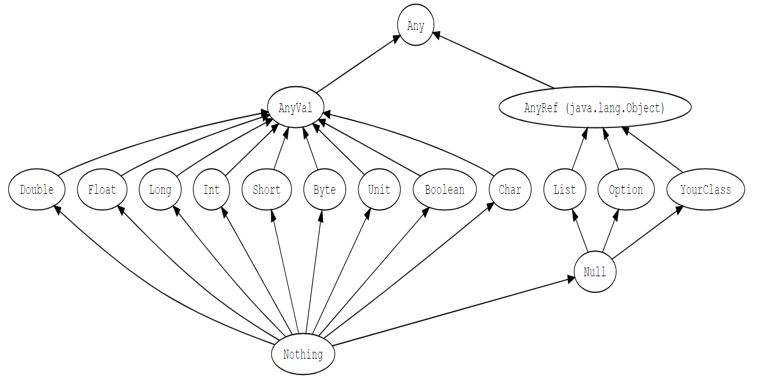
\includegraphics[width=1\textwidth]{pictures/scala-type-hierarchy.jpg}
  \caption{Хијерархија Скала типова}
  \label{fig:scala_types_hier}
\end{figure}

\section{Скала колекције}
\label{sec:scala_coll}

Скала поседује велики број уграђених колекција, мутабилних и имутабилних. Неке од њих су низови, листе, скупови и мапе.

\subsection{Низови}
\label{subsec:scala_arrays}

Скала низ (енг. \textit{array}) је мутабилна структура која представља низ података. Мутабилна је у смислу да се вредности елемената у низу могу мењати, док је број елемената фиксан. Сваки низ садржи елементе једног типа и може се креирати навођењем иницијалних елемената или његове дужине. Уколико се наведе дужина, сви елементи ће бити иницијализовани на подразумевану вредност жељеног типа. \cite{scala_prog}

\begin{lstlisting}[language=Scala, caption={Инстанцирање низа у Скали}, label={lst:scala_coll_array_example}]
scala> val a1 = Array(1, 2, 3)
val a1: Array[Int] = Array(1, 2, 3)

scala> val a2 = new Array[Int](3)
val a2: Array[Int] = Array(0, 0, 0)
\end{lstlisting}

У претходном примеру се у другом случају инстанцира нова класа коришћењем наредбе \textit{new} док у првом то није случај. Разлог је тај што се у првом случају позива метод \textit{apply()} који креира инстанцу низа. Поред тога, у првом случају је Скала компајлер аутоматски закључио тип низа на основу прослеђених елемената, док је у другом тип морао бити експлицитно назначен. \cite{scala_prog}

Елементу низа се приступа слично као у Јави, са тим што се уместо угластих заграда користе обичне. На сличан начин се извршава и мењање једног елемента.

\begin{lstlisting}[language=Scala, caption={Приступ и измена елемента низа}, label={lst:scala_coll_array_get_set}]
scala> val a = Array(1, 2, 3)
val a: Array[Int] = Array(1, 2, 3)

scala> a(0)
val res0: Int = 1

scala> a(0) = 100

scala> a
val res1: Array[Int] = Array(100, 2, 3)
\end{lstlisting}

\subsection{Листе}
\label{subsec:scala_lists}

Скала листе представљају имутабилну колекцију елемената истог типа. Разлика листе у Скали у односу на Јавину је та што је Скала листа увек имутабилна, док Јава листа може бити мутабилна. 

Инстанцира се навођењем елемената. Приступ елементу листе се извршава на исти начин као и у случају низа. Пошто су листе имутабилне, измена вредности елемената није дозвољена. \cite{scala_prog}

\begin{lstlisting}[language=Scala, caption={Пример Скала листе}, label={lst:scala_coll_lists_example}]
scala> val l = List("a", "b", "c")
val l: List[String] = List(a, b, c)

scala> l(0)
val res0: String = a

scala> l(0) = "try"
       ^
       error: value update is not a member of List[String]
       did you mean updated?
\end{lstlisting}

Спајање листи се извршава оператором $:::$. Приликом позива овог оператора се не извршава додавање елемената једне листе на другу, већ је резултат нова листа. Овај метод се може користити и за спајање више од две листе. \cite{scala_prog}

\begin{lstlisting}[language=Scala, caption={Спајање листи}, label={lst:scala_coll_lists_new_list}]
scala> val l1 = List(1, 2, 3)
val l1: List[Int] = List(1, 2, 3)

scala> val l2 = List(4, 5, 6)
val l2: List[Int] = List(4, 5, 6)

scala> val l3 = List(7, 8, 9)
val l3: List[Int] = List(7, 8, 9)

scala> l1 ::: l2 ::: l3
val res0: List[Int] = List(1, 2, 3, 4, 5, 6, 7, 8, 9)
\end{lstlisting}

Нове листе се могу инстанцирати и коришћењем оператора $::$, који као аргументе прима елемент и листу истог типа од којих конструише нову листу где елемент додаје на почетак листе.

\begin{lstlisting}[language=Scala, caption={Пример оператора ::}, label={lst:scala_coll_lists_head_op}]
scala> val l = List(1, 2, 3)
val l: List[Int] = List(1, 2, 3)

scala> 10 :: l
val res0: List[Int] = List(10, 1, 2, 3)
\end{lstlisting}

Коришћењем овог оператора се може извршити надовезивање елемената на празну листу (пример \ref{lst:scala_coll_lists_head_op_nill}). У Скали се празна листа означава кључном речи \textit{Nil}.

\begin{lstlisting}[language=Scala, caption={Додавање елемената на празну листу}, label={lst:scala_coll_lists_head_op_nill}]
scala> val l = 1 :: 2 :: 3 :: 4 :: Nil
val l: List[Int] = List(1, 2, 3, 4)
\end{lstlisting}

\subsection{Н-торке}
\label{subsec:scala_tuple}

Имутабилна колекција која садржи елементе различитог типа се назива н-торка (енг. \textit{Tuple}). Ова структура података се може користити када је потребно вратити више различитих вредности функције. \textit{Tuple} се инстанцира навођењем елемената између заграда. Елементу се приступа оператором \_Х где је \textit{Х} редни број елемента унутар н-торке. \cite{scala_prog}

\begin{lstlisting}[language=Scala, caption={Н-торка у Скали}, label={lst:scala_coll_tuple_example}]
scala> val t = (1, "string123", Array(1, 2, 3))
val t: (Int, String, Array[Int]) = (1,string123,Array(1, 2, 3))

scala> t._1
val res0: Int = 1

scala> t._3
val res1: Array[Int] = Array(1, 2, 3)
\end{lstlisting}

\subsection{Скупови}
\label{subsec:scala_sets}

Скуп је колекција за коју важи да садржи елементе истог типа, са тим што сваки елемент колекције мора бити јединствен. Постоје две врсте скупова, имутабилни (\textit{collection.immutable.Set}) и мутабилни (\textit{collection.mutable.Set}).

Инстанцирају се на исти начин као и низ, навођењем елемената. Уколико се током навођења наведе неки елемент више од једног пута, не добија се грешка, већ се дупликат аутоматски уклања. Елемент се додаје оператором $+$. Код мутабилних скупова $+$ додаје елемент на постојећи скуп, док код имутабилних производи нови скуп са додатим елементом. \cite{scala_prog}

\begin{lstlisting}[language=Scala, caption={Инстанцирање скупа у Скали}, label={lst:scala_coll_set_example}]
scala> val s = Set(1, 1, 1, 1, 2, 2)
val s: scala.collection.immutable.Set[Int] = Set(1, 2)
\end{lstlisting}

\subsection{Мапе}
\label{subsec:scala_maps}

Мапе су колекције за рад са кључ-вредност паровима. Постоје мутабилне (\textit{collection.mutable.Map}) и имутабилне (\textit{collection.immutable.Map}). Имутабилне су подразумеване и користе се уколико се експлицитно не наведе супротно.

Дефинишу се навођењем низа кључ-вредност парова, раздвојених знаком $->$. Сви кључеви и све вредности међусобно морају бити истог типа. Приступ вредностима се врши преко назива кључа, методом $()$.

\begin{lstlisting}[language=Scala, caption={Мапе у Скали}, label={lst:scala_app_maps_example}]
scala> val m1 = Map("k1" -> "v1", "k2" -> "v2")
val m1: scala.collection.Map[String,String] = Map(k1 -> v1, k2 -> v2)

scala> m1("k1")
val res0: String = v1

scala> val m2 = Map(1 -> Array(1, 2), 2 -> Array(3, 4))
val m2: scala.collection.Map[Int,Array[Int]] = Map(1 -> Array(1, 2), 2 -> Array(3, 4))

scala> m2(1)
val res1: Array[Int] = Array(1, 2)
\end{lstlisting}

Разлика између мутабилних и имутабилних мапа је та што је код мутабилних могуће изменити број елемената, као и саме елементе, док имутабилна мапа то не подржава.

\begin{lstlisting}[language=Scala, caption={Измена и додавање елемента код мутабилних и имутабилних мапа}, label={lst:scala_coll_maps_mutable_immutable}]
// mutable map
scala> val mutableM = mutable.Map("k1" -> "v1")
val mutableM: scala.collection.mutable.Map[String,String] = HashMap(k1 -> v1)

scala> mutableM("k1") = "vred1"

scala> mutableM("k2") = "vred2"

scala> mutableM
val res0: scala.collection.mutable.Map[String,String] = HashMap(k1 -> vred1, k2 -> vred2)

// immutable map
scala> val immutableM = Map("k1" -> "v1")
val immutableM: scala.collection.Map[String,String] = Map(k1 -> v1)

scala> immutableM("k1") = "vred1"
       ^
       error: value update is not a member of scala.collection.Map[String,String]

scala> immutableM("k2") = "vred2"
       ^
       error: value update is not a member of scala.collection.Map[String,String]

\end{lstlisting}

\section{Поклапање образаца}
\label{sec:scala_patt_match}

Поклапање образаца (енг. \textit{pattern matching}) је честа карактеристика функционалних језика. Слична је наредби \textit{switch} из Јаве, али нуди више могућности од ње. Састоји се од селектора, који представља израз или променљиву, кључне речи \textit{match} и низа случајева унутар витичастих заграда. Сваки случај се састоји од знака $=>$ који се налази између вредности са којом се селектор поклапа и кључне речи \textit{case} са леве стране и израза који ће бити резултат поклапања са десне. \cite{scala_prog}

\begin{lstlisting}[language=Scala, caption={Поклапање образаца у Скали}, label={lst:scala_coll_patt_match}]
selector match {
	case value1 => result1
	case value2 => result2
	case value3 => result3
	...
}
\end{lstlisting}

Разлике између ове нарeдбе и Јавине наредбе \textit{switch} су:

\begin{itemize}
\item \textit{match} наредба увек резултује неком вредношћу
\item Када се пронађе одговарајућа вредност, друге вредности након ње се не разматрају. Није потребно користити наредбу \textit{break}
\item Уколико ниједна вредност не одговара селектору, појављује се \textit{MatchError}. То значи да увек треба покрити све могуће вредности селектора
\end{itemize}

\subsection{Примери коришћења}
\label{subsec:scala_match_exaples}

Поклапање образаца је веома моћан механизам и користи се у великом броју случајева. Један од њих је поклапање константи:

\begin{lstlisting}[language=Scala, caption={Поклапање константи}, label={lst:scala_patt_match_match_const_example}]
scala> def describe(x: Any) = x match {
     | case 5 => "five"
     | case true => "truth"
     | case "hello" => "hi!"
     | case Nil => "the empty list"
     | case _ => "something else"
     | }
     
scala> describe(5)
val res1: String = five

scala> describe(Nil)
val res2: String = the empty list

scala> describe(1001)
val res3: String = something else
\end{lstlisting}

У претходном примеру се у последњем случају користи ознака $\_$. Назива се џокер (енг. \textit{wildcard}) и поклапа се са било којом вредношћу селектора.

\begin{lstlisting}[language=Scala, caption={Џокер у поклапању образаца}, label={lst:scala_patt_match_wildcard}]
scala> def describe(x: Int) = x match {
     | case 10 => "x je 10"
     | case _ => "x nije 10"
     | }
def describe(x: Int): String

scala> describe(10)
val res1: String = x je 10

scala> describe(100)
val res2: String = x nije 10

scala> describe(-100)
val res3: String = x nije 10
\end{lstlisting}

Поклапање образаца се користи и за поклапање променљивих. У примеру \ref{lst:scala_patt_match_variable_match_example} променљива \textit{something} одговара било којој вредности селектора, слично као џокер, али се преко ње та вредност преноси са десне стране ознаке $=>$. \cite{scala_prog}

\begin{lstlisting}[language=Scala, caption={Поклапање променљивих}, label={lst:scala_patt_match_variable_match_example}]
scala> val expr = "some expression"
val expr: String = some expression

scala> expr match {
     | case ""        => print("empty string")
     | case something => print("matched: " + something)
     | }
matched: some expression
\end{lstlisting}

Поред вредности селектора, могуће је поклапати и његов тип, уколико је потребно имплементирати другачије понашање за другачије типове .

\begin{lstlisting}[language=Scala, caption={Поклапање типова}, label={lst:scala_patt_match_types_example}]
scala> trait MyTrait
trait MyTrait

scala> class MyClass_1 extends MyTrait
class MyClass_1

scala> class MyClass_2 extends MyTrait
class MyClass_2

scala> def describe(x: MyTrait) = x match {
     |   case mc1: MyClass_1 => "MyClass_1"
     |   case mc2: MyClass_2 => "MyClass_2"
     |   case _ => "some other class"
     | }
def describe(x: MyTrait): String

scala> describe(new MyClass_1)
val res1: String = MyClass_1

scala> describe(new MyClass_2)
val res2: String = MyClass_2
\end{lstlisting}

Могуће је комбиновати претходне примере и извршити поклапања типова и променљивих уз помоћ једног поклапања образаца. Пример \ref{lst:scala_patt_match_generalSize} приказује функцију \textit{generalSize(x: Any)} која се понаша другачије у односу на то ког типа је њен аргумент. \cite{scala_prog}

\begin{lstlisting}[language=Scala, caption={Пример поклапања типова и променљивих}, label={lst:scala_patt_match_generalSize}]
scala> def generalSize(x: Any) = x match {
     |   case s: String => s.length
     |   case m: Map[_, _] => m.size
     |   case _ => -1
     |  }
def generalSize(x: Any): Int

scala> generalSize("some string")
val res1: Int = 11

scala> generalSize(12)
val res2: Int = -1
\end{lstlisting}

Поклапање конструктора се користи када је потребно извршити поклапање класа које наслеђују заједничку класу. 

\begin{lstlisting}[language=Scala, caption={Поклапање конструктора}, label={lst:scala_patt_match_constr_match_example}]
scala> abstract class Animal
     | case class Mammal(name: String) extends Animal
     | case class Bird(name: String) extends Animal
class Animal
class Mammal
class Bird

scala> def caseClassesPatternMatching(animal: Animal) = animal match {
     |  case Mammal(name) => s"I'm a $name, a mammal"
     |  case Bird(name) => s"I'm a $name, a bird"
     |  case _ => "I'm an unknown animal"
     |}
def caseClassesPatternMatching(animal: Animal): String
\end{lstlisting}

%\section{Optional и Either}
%\label{sec:scala_opt_eith}=
%optional i either tipovi

%\section{Implicit vred}
%\label{sec:scala_impl_vals}
%implicits
%if requested

\chapter{Дистрибуирани системи}
\label{chp:dist_sis}

\section{Увод}
\label{sec:uvod}

У данашње време се генерише огромна количина података. Друштвене мреже, видео садржај и куповина преко интернета су само неке од ствари које на дневном нивоу производе петабајте података, а у будућности се очекује пораст тог тренда.

Према истраживању приказаном на једном од водећих интернет платформи за податке који се користе у пословању, количина података који производимо се тренутно може мерити у десетинама зетабајта (енг. \textit{zetabyte}) \footnote{милијарда терабајта}. Исто истраживање приказује да ће се наредних година тај број удвостручити. \cite{volume_data}

\begin{figure}[!ht]
  \centering
  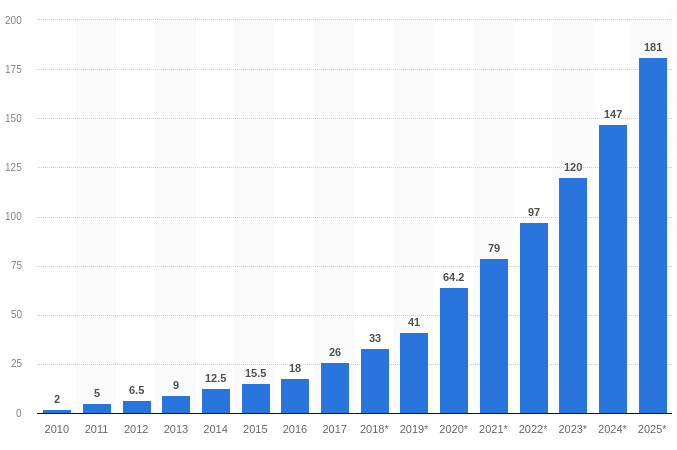
\includegraphics[width=0.8\textwidth]{pictures/Total_data_volume_worldwide_2010_2025_statista.png}
  \caption{количина података по години у зетабајтима}
  \label{fig:kolicina_podataka}
\end{figure}

Корист података је огромна и велики број индустрија и компанија их користи на разне начине, од побољшања искуства корисника који користе њихове услуге, до разних предвиђања у пословању. Из тих разлога се доста улаже у складиштење, обраду, истраживање и анализу података.

Раније су подаци, док још увек нису генерисани у количинама у којима се то дешава данас, обрађивани на појединачним машинама, али се убрзо испоставило да такав приступ има своје лимите.

\section{Скалирање система}
\label{sec:skaliranje}

Постоје два начина скалирања уређаја који врше обраду података. Први начин је вертикално скалирање (енг. \textit{vertical scaling} или \textit{scale-up}). У овом приступу ми унапређујемо једну машину, на пример додајемо јој више меморије или појачавамо снагу процесора. Предности овог приступа је то што након што унапредимо машину не морамо да мењамо логику апликација које се на њој извршавају. Али негативне ствари су те што постоји некакво ограничење до ког можемо унапредити машину (ипак морамо обрадити егзабајте података), као и то да морамо да обратимо посебну пажњу на то шта се дешава ако систем доживи некакву грешку и неочекивано престане са радом. \cite{hadoop_beginner}

Други приступ је хоризонтално скалирање (енг. \textit{horizontal scaling} or \textit{scale-out}). У овом случају не унапређујемо једну машнину, већ, уколико нам је потребна додатна снага, додајемо нову машину у систем. Добра ствар је та што је често јефтиније додати неколико нових машина у систем него унапредити процесор неколико пута на истој машини. Још једна веома добра ствар је ефикасност. Када имамо неколико машина можемо на свакој од њих обрађивати један део података, што је огромна предност у односу на вертикално скалирање. Међутим, хоризонтално скалирање доноси додатан скуп проблема. Потребно је имплементирати цео систем, омогућити машинама да раде заједно и координисати их, као и обрадити проблеме који се могу десити на појединачним машинама. \cite{hadoop_beginner}

Због наведених предности и мана, данашњи стандард у обради података је хоризонтално скалирање.

\begin{figure}[!ht]
  \centering
  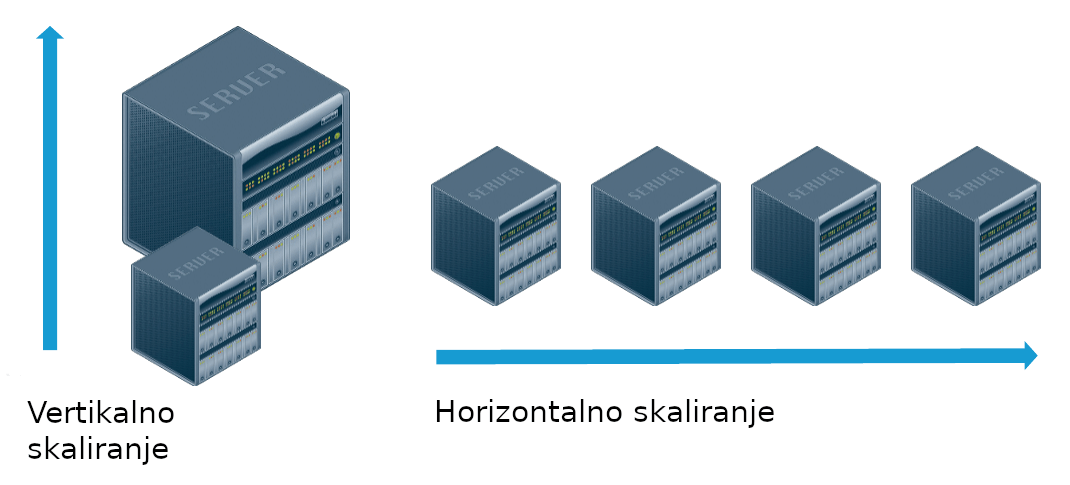
\includegraphics[width=0.8\textwidth]{pictures/scaling.png}
  \caption{Врсте скалирања}
  \label{fig:skaliranje}
\end{figure}

\section{Особине дистрибуираних система}
\label{sec:scaling_osobine}

Идеја је да свака машина у систему обрађује један део података и да на тај начин допринесе коначном резултату. То значи да машине морају да комуницирају једна са другом и да ће неки подаци можда затребати свакој машини у систему. То може довести до тога да се уређаји такмиче међу собом за приступ подацима. Такође, уколико се подаци налазе само на једној машини у систему, све друге машине ће јој приступити, тако да су могућности нашег система у том случају ограничене могућностима те једне машине којој сви приступају. Поред тога, та машина може да доживи некакав проблем и да због тога престане да функционише, што би изазвало престанак рада целог система. \cite{hadoop_beginner}

Због тога, систем би требало да функционише тако да уређаји који су у њему раде независно од других уређаја истог система, као и да престанак рада једне машине не утиче на систем у целини. Другим речима, требало би направити такав систем који очекује да се фаталне грешке дешавају. У овим системима је акценат на софтверу, а не на хардверу. Наиме, идеја је да се систем може направити од уређаја који су масовно доступни. Такође, идеја је да се избегава трансфер података међу уређајима. Дакле, подаци би, уколико је то могуће, требало да се обрађују на машини на којој се налазе. \cite{hadoop_beginner}

\section{Хадуп}
\label{sec:hadoop}

Први успешан систем који поседује претходно наведене карактеристике је остварила компанија Гугл (енг. \textit{Google}) која је 2003. године објавила научни рад на ту тему. У том научном раду је представљен дистрибуирани фајл систем, назван Гугл фајл систем (енг. \textit{Google file system}) или скраћено ГФС (енг. \textit{GFS}). Идеја иза овог пројекта написаног у програмском језику \textit{C++} је да се користи за складиштење великих количина података. \cite{gfs}

Већ следеће године, Гугл је објавио нови научни рад о парадигми за ефикасну обраду велике количине података на кластеру. Парадигма је названа Мап редјус (eng. \textit{Map Reduce)} и њена намена је да се користи за обраду података складиштених у ГФС-у. \cite{gmr}

Недуго након тога, уз помоћ научних радова компаније Гугл, настао је пројекат отвореног кода (енг. \textit{Open source}) назван Хадуп (енг. \textit{Hadoop}) са идејом да имплементира карактеристике које имају гуглови ГФС и Мап Редјус и да се као такав користи за складиштење и ефикасну обраду падатака на кластеру сачињеном од релативно јефтиних машина. Највећи делови Хадупа су ХДФС (енг. \textit{HDFS}) и Мап редјус (енг. \textit{Map Reduce}), скраћено МР (енг. \textit{MR}) који су заправо јавно доступни еквиваленти Гуглових технологија. \cite{hadoop_beginner}

Укратко, ХДФС је фајл систем који користи хоризонтално скалирање машина за складиштење огромних количина података. Због боље поузданости користи репликацију, где се сваки фајл копира неколико пута и онда се те копије чувају на различитим уређајима у систему. \cite{hadoop_beginner}

МР је парадигма за обраду података, која се састоји из два дела названа Мап (енг. \textit{map}) и Редјус (енг. \textit{reduce}), по којима је парадигма и добила име. У оба дела се над подацима који се налазе у ХДФС-у врши некаква обрада података. Напоменимо да се и сама обрада извршава на ХДФС-у, на истом месту где се подаци и налазе, дакле избегава се беспотребно премештање на неку другу машину. \cite{hadoop_beginner}

Обе компоненте су направљене да функционишу на релативно јефтином, обичном хардверу. Поред тога користе хоризонтално скалирање и у стању су да наставе са радом чак и ако једна или више машина у систему из неког разлога престане да функционише.

\begin{figure}[!ht]
  \centering
  
\includegraphics[width=0.8\textwidth]{pictures/hdfs_mr_logo.png}
  \caption{ХДФС и МР}
  \label{fig:hdfs_mr_logo}
\end{figure}

Поред поменуте две компоненте, постоји и трећа, а то су ХДФС апликације. Оне се надовезују на ХДФС и МР тако што их користе за редом складиштење и обраду. Најпознатије од њих су Хајв (енг. \textit{Hive}) и Пиг (енг. \textit{Pig}), али поред њих наравно постоје и многе друге, само мање заступљене. На слици \ref{fig:hadoop_aplikacije} можемо видети компоненте Хадупа. \cite{hadoop_learning}

\begin{figure}[!ht]
  \centering
  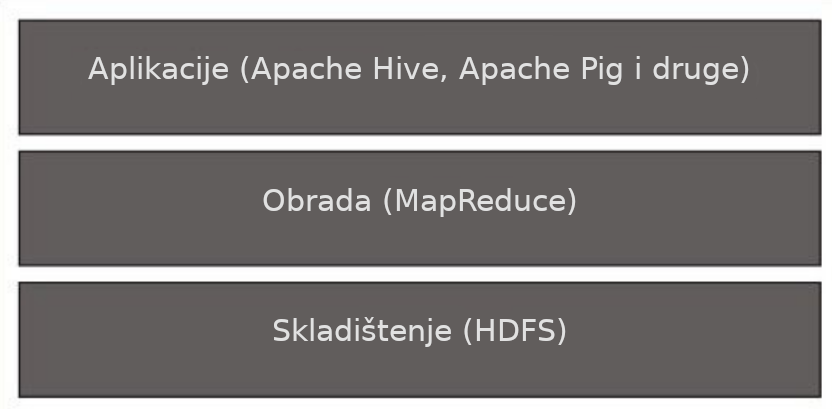
\includegraphics[width=0.8\textwidth]{pictures/hadoop_apps.png}
  \caption{Упрошћен приказ Хадупа}
  \label{fig:hadoop_aplikacije}
\end{figure}


\section{ХДФС}
\label{sec:hdfs}

ХДФС, скраћено од Хадупов дистрибуирани фајл систем (енг- \textit{Hadoop distributed file system}) је, као што му је у имену и написано, дистрибуирани систем, што значи да складишти податке на више машина које ћемо у даљем тексту звати чворови (енг. \textit{nodes}). 

\subsection{Врсте уређаја ХДФС-а}
\label{subsec:hdfs_nodes}

Постоје две врсте чворова, именски (енг. \textit{name node}) и дата (енг. \textit{data node}) (слика \ref{fig:hadoop_nodovi}). Сваки ХДФС систем има један именски чвор чија је улога да управља фајл системом и да регулише приступ подацима који се налазе на њему. Он садржи информације о фајловима, као што су између осталих име, локација у систему где се фајл налази, последњи датум промене фајла као и правила приступа. \cite{hadoop_arch_guide}

Друга врста је дата чвор и њих се у систему обично налази више од једног. На њима се заправо складиште фајлови у систему али се поред тога користе и за компутације. Такође, дата чворови су задужени за операције над фајловима као што су читање, мењање и брисање. Они ће урадити неку од тих операција само када им именски чвор то нареди. \cite{hadoop_arch_guide}

Уколико имамо неког клијента који жели да приступи ХДФС-у, он ће прво комуницирати са именским чвором и од њега затражити фајлове који му требају. Након тога ће именски чвор проверити да ли клијент има потребне пермисије и ако их има, послаће му локацију фајла у фајл систему. Тек након тога се може извршити жељени приступ. 

\begin{figure}[!ht]
  \centering
  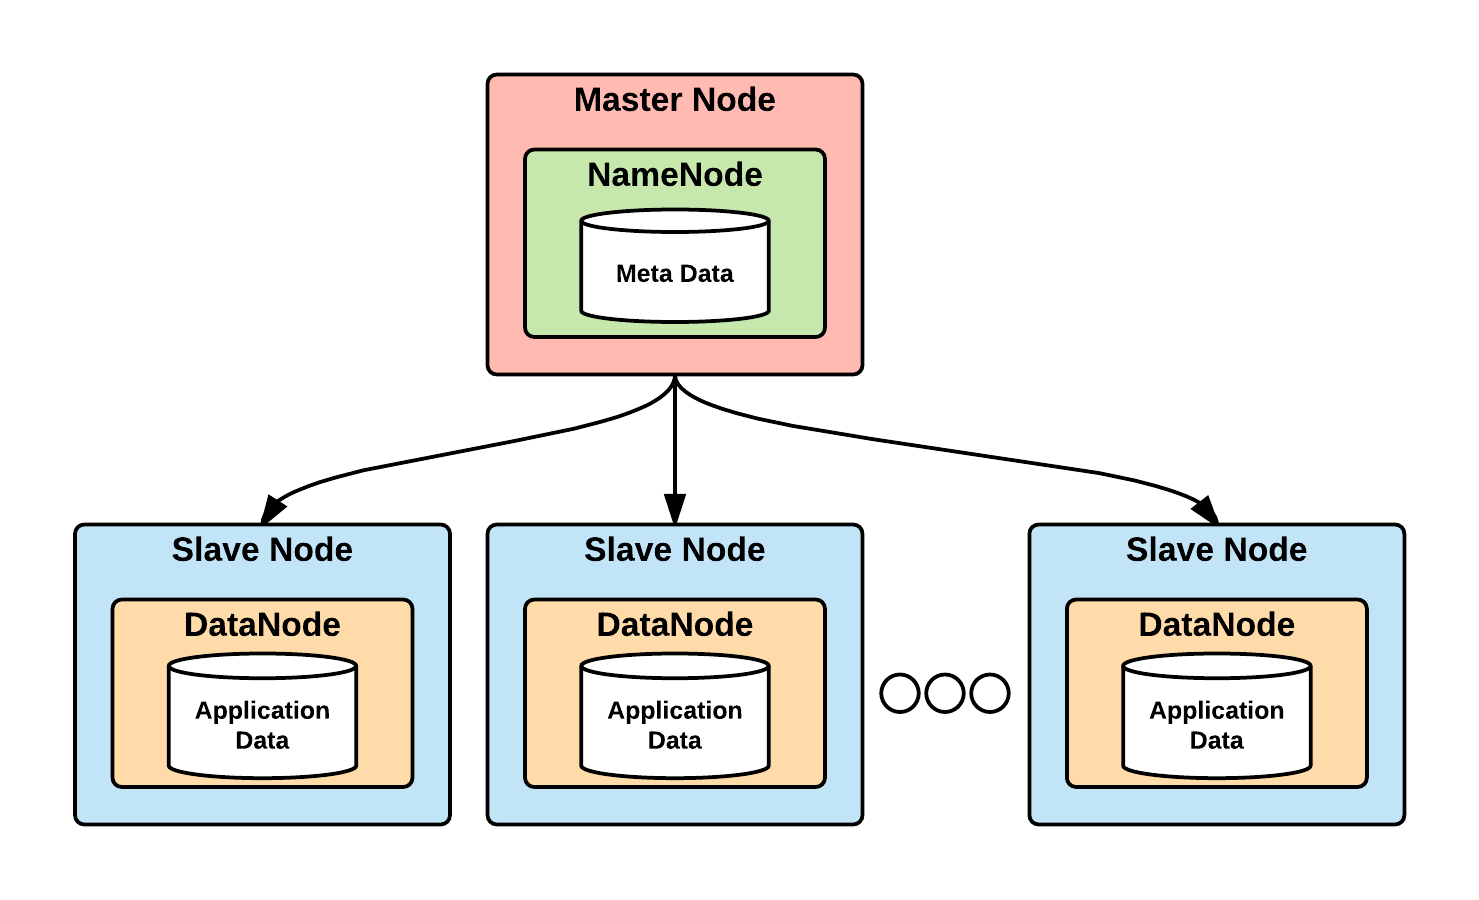
\includegraphics[width=0.9\textwidth]{pictures/hdfs_nodovi.png}
  \caption{Врсте чворова у ХДФС-у}
  \label{fig:hadoop_nodovi}
\end{figure}

\subsection{Особине}
\label{subsec:hdfs_osobine}

Сваки фајл у ХДФС-у је подељен на делове које зовемо блокови, чија је величина обично 128 мегабајта. Блокови се често не налазе на истим чворовима у систему, што значи да један фајл чувамо на неколико физички раздвојених машина. Ту може да настане проблем због тога што једна од тих машина може да се поквари и због тога престане са радом. Ако се то деси, сви блокови на тој машини ће нестати. ХДФС очекује ово и због тога се сваки блок реплицира неколико пута и онда се оригинални блок и његове реплике распореде по систему. Ако један од блокова фајла неочекивано нестане, увек можемо приступити једној од његових реплика. Напоменимо још једном да ће се реплике чувати на дата чворовима, док ће се информације о томе ком фајлу реплике припадају налазити на именским чвору. \cite{hadoop_arch_guide}

Блок ће се увек реплицирати одређен, фиксан, број пута. Дата чворови повремено шаљу сигнале именском чвору о доступности реплика. На тај начин ће именски чвор увек знати колико је пута сваки блок реплициран у систему и на основу тога може да, уколико тај број падне испод неког задовољавајуће вредности, направи нове реплике тог блока. \cite{hadoop_arch_guide}

Поменули смо да ХДФС очекује пад дата чворова и губитак података на њима. Али шта се дешава ако се проблем деси на најбитнијем чвору у систему, именском, и он неочекивано престане са радом? Такви проблеми се заобилазе тако што се чувају резервне копије именског чвора због којих се и у случају престанка његовог рада не губе никакве информације. Напоменимо да се резервне копије праве у одређеним временским интервалима да би подаци на њима били ажурни. Поменути концепти су приказани на слици \ref{fig:hadoop_sistem}.

\begin{figure}[!ht]
  \centering
  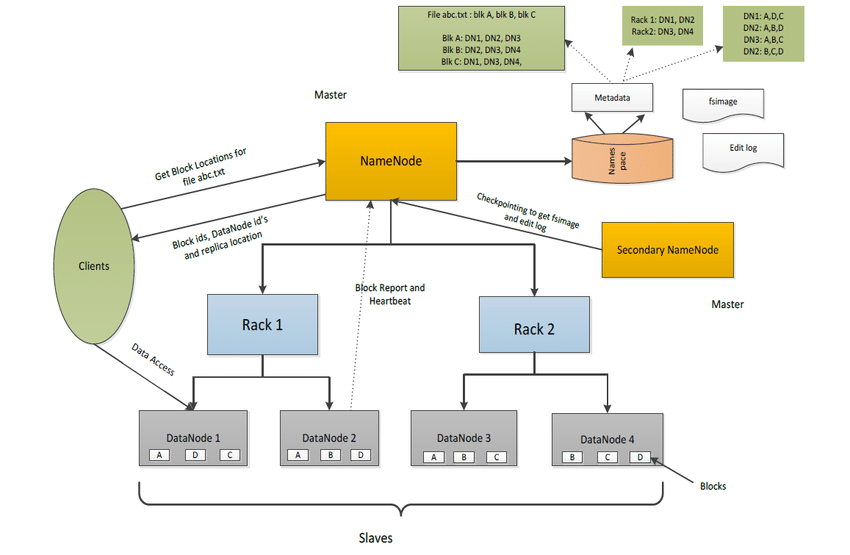
\includegraphics[width=1\textwidth]{pictures/hadoop_system.png}
  \caption{ХДФС компоненте}
  \label{fig:hadoop_sistem}
\end{figure}

Претходно поменуте особине су битне за целокупну робусност система, односно поузданости података чак и у случајевима када се десе некакви проблеми.

ХДФС је систем за кога важи пиши једном, читај више пута (енг. \textit{write-once, read-many (WORM)}). Дакле, када поставимо фајл на ХДФС не можемо га мењати. Ако желимо да променимо фајл морамо да поставимо тотално нови фајл уместо старог. Иако то није ефикасно, то често није битно због тога што се апликације које обрађују велике количине података заснивају на томе да се подаци не мењају, па је за очекивати да за променама неће бити ни потребе или се то барем неће често дешавати. \cite{hadoop_beginner}

% https://www.quora.com/Is-HDFS-an-append-only-file-system-Then-how-do-people-modify-the-files-stored-on-HDFS.

Такође, још једна од особина ХДФС-а је та да је конструисан да има добре перформансе у случајевима када нам је потребан велики проток података, на пример у случају читања великих фајлова. \cite{hadoop_beginner}


\section{Мап Редјус}
\label{sec:mr}

Као што је већ наведено, МР је парадигма која се користи за обраду података који су складиштени у ХДФС-у. Користи подели и завладај (енг. \textit{divide and conquer}) приступ приликом обраде података са идејом да више машина паралелно обрађује један њихов део. На тај начин се, на пример, обрада података која би трајала 1000 минута, ако се паралелизује на 1000 машина, могла свести на обраду која траје само један минут. \cite{hadoop_beginner}

Парадигма је заснована на концептима из функционалног програмирања и функцијама које се често користе у обради низова и листи. Те фунције се зову мап и редујс. Прва од постојеће листе креира нову тако што на сваки елемент листе примени неку фунцију и од њега направи нови елемент. Друга од целе листе конструише једну вредност. На истим принципима фунционише и мап редјус парадигма.

МР обрађује податке у неколико фаза. Прво, подаци се читају из ХДФС-а и након тога се прослеђују машинама које називамо мапери (енг. \textit{mappers}). Те машине паралелно производе скуп привремених података који се након тога распоређују, сортирају и шаљу машинама које називамо редјусери (енг. \textit{reducers}). Фаза која распоређује податке се назива фаза мешања и сортирања (енг. \textit{shuffle and sort}). Задатак редјусера је да приме некакав скуп података и да паралелно произведу једну вредност од истих. На самом крају се резултат свих редјусера комбинује и добија се резултат читавог МР процеса, другачије названог и МР задатак (енг. \textit{task}). Напоменимо да је могуће комбиновати МР задатке тако да излаз из једног буде улаз у други. \cite{hadoop_learning}

\subsection{Мап Редјус из аспекта функција}
\label{subsec:mr_funck_asp}

Из функционалног аспекта, мап и редјус фазе можемо посматрати на следећи начин. Нека имамо листу почетних података у (кључ, вредност) формату. Због једноставности ћемо за поменути формат користити ознаку (к, в). Дакле, током мап фазе се подаци из листе парова читају, деле у мање подлисте на које се паралелно примењује мап функција коју дефинишемо. Паралелизам се постиже тако што се свака подлиста обрађује на засебној машини (маперу). Мап фаза као улаз прима листу (к, в) парова и производи нову листу истог формата. \cite{hadoop_learning}

$$ list(k1, v1) -> map(k1, v1) -> list(k2, v2) $$

Након тога се те нове листе групишу тако што се за сваки кључ прави једна група која ће бити процесуирана од стране једне машине (редјусер). Дакле, није могуће да се подаци који имају различите кључеве нађу на истој машини у истом тренутку. Тај већ поменути део обраде је \textit{shuffle and sort}. 

$$ list(k2, v2) -> shuffleAndSort(k2, v2) -> k2, list(v2) $$

На крају се на сваку од група паралелно примењује редјус функција која производи једну вредност за сваку групу. Дакле редјус прима кључ и листу вредности које му одговарају и као резултат производи једну вредност формата (кључ, вредност). \cite{hadoop_learning}

$$ k2, list(v2) -> reduce(k2, list(v2)) -> (k3, v3) $$

Тако добијен резултат се уписује у ХДФС. Цео процес је приказан на слици \ref{fig:map_reduce} где је као пример представљена МР апликација која пребројава број појављивања сваке речи у тексту. \cite{hadoop_learning}

\begin{figure}[!ht]
  \centering
  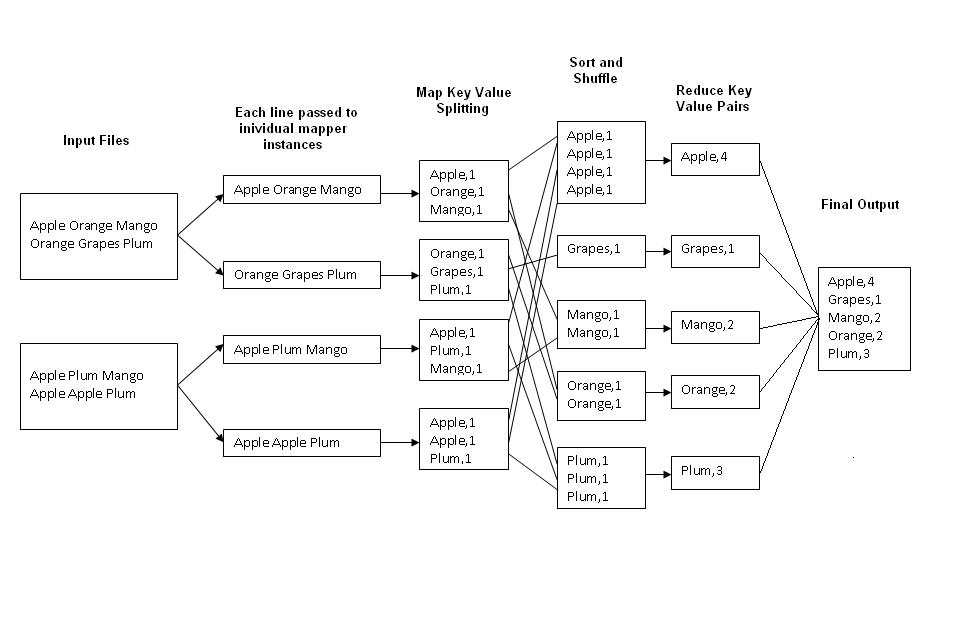
\includegraphics[width=1\textwidth]{pictures/mapreduce_step2.jpg}
  \caption{Пример МР апликације}
  \label{fig:map_reduce}
\end{figure}

У МР апликацијама задатак програмера је да опише како ће се извршавати мап и редјус фазе, док ће се Хадуп систем побринути за све остало: читање података, сортирање, паралелизацију, координацију и извршавање послова. \cite{hadoop_beginner}

Напоменимо и то да је ова парадигма направљена да ради за податке у (кључ, вредност) формату, а не за податке који имају дефинисану шему. Пример података који имају шему би биле табеле у релационим моделима. \cite{hadoop_beginner}


\section{Остале компоненте Хадупа}
\label{sec:ostale_komp_hadupa}

У овој секцији ћемо само напоменути неке од технологија које користе ХДФС и које заједно са њим чине Хадуп екосистем (енг. \textit{Hadoop ecosystem}). Те технологије имају широке области примене. Неке од њих су преговарач ресурса Јарн (енг. \textit{Yarn}) о коме ћемо у више детаља писати у следећој секцији, Кафка (енг. \textit{Kafka}), апликација која ради над токовима података, Пиг (енг. \textit{Pig}) и Хајв (енг. \textit{Hive}) које су намењене за обраду података и имплементиране су користећи МР. Поред њих постоје и многе друге, као на пример Престо (енг. \textit{Presto}), Xjу (енг. \textit{Hue}), Флум (енг. \textit{Flume}) и друге, али оне, као ни операције за које су намењене, нису фокус овог рада. Приказ малог дела Хадуп екосистема је приказан на слици \ref{fig:hadoop_ecosystem}.


\begin{figure}[!ht]
  \centering
  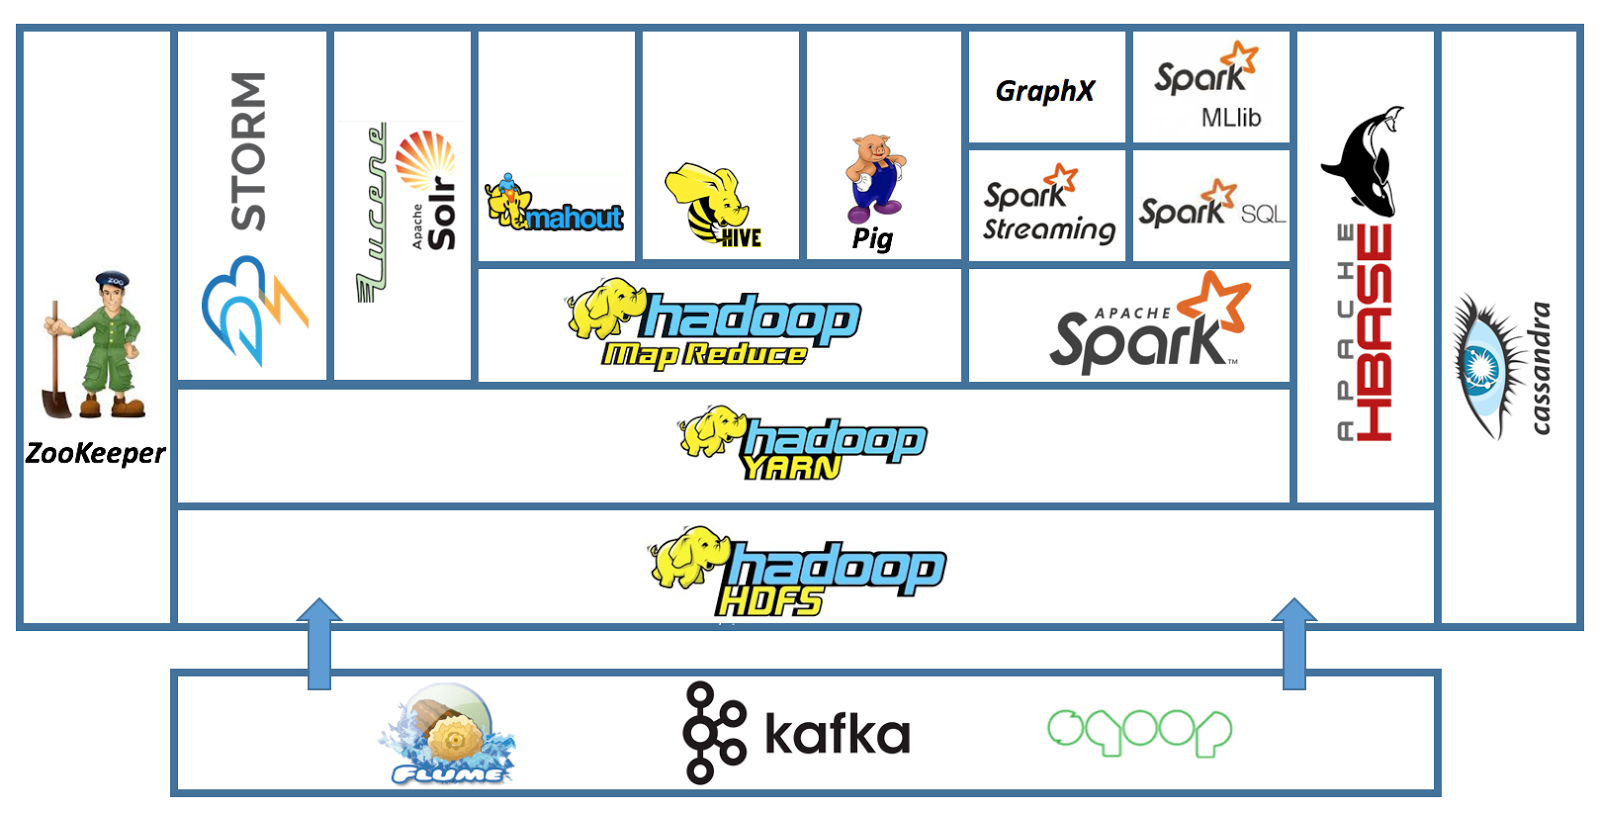
\includegraphics[width=1\textwidth]{pictures/hadoop_ecosystem.png}
  \caption{Хадуп екосистем}
  \label{fig:hadoop_ecosystem}
\end{figure}


\section{Апачи Јарн}
\label{sec:yarn}

У првој верзији Хадупа, мап редјус је заправо имао две намене. Прва је била већ поменута обрада велике количине података за коју је МР примарно и намењен, док је друга била алокација и управљање ресурсима који су МР апликацији били потребни као и заказивање МР таскова. Такав систем је конструкцију апликације које користе МР учинио веома тешким. Због тога је одлучено да МР буде намењен само обради података, док је друга улога дата другој апликацији коју би МР користио. \cite{hadoop_learning}

Резултат је менаџер ресурса (енг. \textit{resource manager}) отвореног кода назван Јарн (енг. \textit{Yarn, yet another resource negotiator}) који распоређује таскове апликација које користе Хадуп, али и алоцира ресурсе који су тим апликацијама потребни. Конструисан је тако да није специфичан само за МР, већ пружа интерфејс ка Хадупу разним апликацијама међу којима је и Спарк, о коме ће пречи бити касније. \cite{hadoop_learning}

\begin{figure}[!ht]
  \centering
  
\includegraphics[width=0.6\textwidth]{pictures/yarn_logo.jpg}
  \caption{Апачи Јарн}
  \label{fig:yarn_logo}
\end{figure}

\subsection{Архитектура Јарна}
\label{subsec:yern_arch}

Као што је већ напоменуто, Јарн се не бави обрадом података, већ му је улога да апликацијама које обрађују податке обезбеди ресурсе потребне за њихово извршавање. Направљен је тако да може да подржи разне врсте апликација. \cite{hadoop_learning}

Конструисан је од две главне компоненте, менаџера ресурса (енг. \textit{resource manager}) у даљем тексту РМ и од менаџера чворова (енг. \textit{node manager}) у даљем тексту НМ. Улога првог је да управља ресурсима кластера, док је намена другог да управља ресурсима машине на којој је покренут. То значи да ће кластер имати један РМ и више НМ. Заједно, они ће управљати контејнерима (енг. \textit{container}), апстракцијом меморије, процесорске снаге и И/O операција потребних да би се извршио један део апликације на кластеру. \cite{hadoop_learning}

Улога Јарна је само да обезбеди ресурсе и распореди извршавање таскова на кластеру. Све остало, попут мониторинга, праћења прогреса апликација, обраде грешака и сличног је имплементирано у коду апликације која га користи. Идеја иза тога је да Јарн буде што је више могуће независан да би различите врсте апликација могле да га користе. \cite{hadoop_learning}

Апликација коју покрећемо преко Јарна се састоји из два дела. Први је код који треба извршити док је други назван мастер апликације (енг. \textit{application master}), даље АМ. Његова улога је да управља апликацијом. Као што је у прошлом пасусу поменуто, Јарн се не бави мониторингом и прогресом апликације која је покренута, већ је то улога саме апликације. То апликација успева да уради преко мастера апликације и Јарн нема информацију о томе на који начин је успостављена комуникације између АМ и кода који се извршава. Приказ архитектуре је приказан на слици \ref{fig:yarn_ar}. \cite{hadoop_learning}

\begin{figure}[!ht]
  \centering
  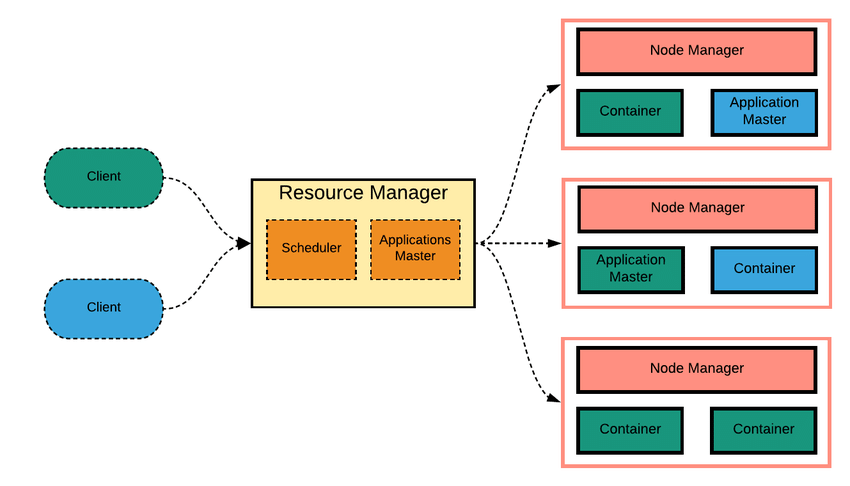
\includegraphics[width=1\textwidth]{pictures/yarn.png}
  \caption{Архитектура Јарна}
  \label{fig:yarn_ar}
\end{figure}

Апликације се, користећи Јарн, на кластеру покрећу преко клијента. Када започнемо Јарн апликацију, клијент прво комуницира са менаџером ресурса и преко њега захтева иницијални контејнер на коме ће покренути мастер апликације. У већини случајева се мастер апликације покреће унутар једног контејнера у кластеру, исто као што се покреће и код саме апликације. Након тога почиње комуникација између покренутог мастера апликације и менаџера ресурса. Та комуникација се одвија тако што АМ захтева од РМ контејнере који су потребни апликацији и менаџер ресурса након тога шаље податке АМ о контејнерима које апликација може да користи. Користећи те информације, АМ комуницира са менаџерима чворова који се налазе на истим машинама као и захтевани контејнери и пружа им спецификације о апликацији која треба да буде покренута у тим контејнерима. Након тога, менаџери чворова започињу извршавање апликације. Од овог тренутка, даље понашање апликације зависи од самог кода те апликације. \cite{hadoop_learning}

Јарн има одговорност да омогући правилно извршавање апликацијама које се извршавају на ХДФС-у па стога мора на неки начин обрадити грешке које се могу десити у кластеру. На пример, за очекивати је да једна од машина у кластеру престане се радом и тако постане неупотребљива. Када се то деси, менаџер ресурса ће менаџер чворова на тој машини означити мртвим и неће га више разматрати. Исто ће се десити и са контејнерима те машине. Такође, сваки контејнер који почне да користи више ресурса од оних који су му омогућени ће бити уништен да не би стварао проблем другим апликацијама у систему. \cite{hadoop_learning}

\section{Апачи Спарк}
\label{sec:spark}

\subsection{Недостаци Мап Редјуса}
\label{subsec:nedost_mr}

Мап Редјус, нажалост, не функционише савршено, што се огледа у проблемима који постоје када су у питању перформансе. Наиме, једна МР апликација је заправо ланац МР послова које треба извршити и сваки од тих послова се састоји из мап и редјус фаза. Излаз једног посла представља улаз у други и тако даље док се не добије коначно решење. Пример једне МР апликације је приказан на слици \ref{fig:mr_app_example}.

\begin{figure}[!ht]
  \centering
  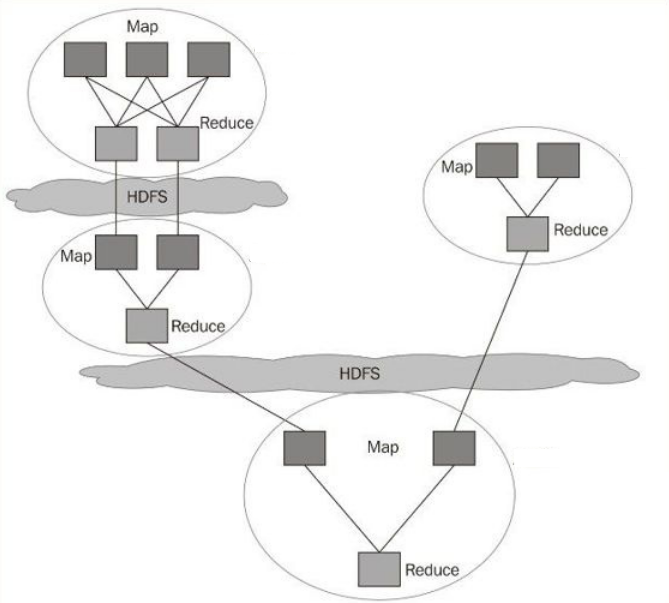
\includegraphics[width=1\textwidth]{pictures/mr_app.png}
  \caption{пример ланца мап редјус послова}
  \label{fig:mr_app_example}
\end{figure}

Међутим, такав приступ има цену а то је да се излаз који генерише један МР посао чува унутар ХДФС-а и одатле ће му приступити остали МР послови којима је тај излаз потребан. Другим речима, међурезултати послова се чувају на диску, што ствара додатне И/О операције и тиме успорава извршавање целокупне апликације. Поред тога, не постоји начин да се ти МР послови на неки начин оптимизују као на пример неком комбинацијом или слично, већ су независни. Да би се решили ови проблеми направљен је нови алат који је данас скоро потпуно избацио МР из употребе, Апачи Спарк (енг. \textit{Spark}). \cite{hadoop_learning}

\subsection{Увод у Апачи Спарк}
\label{subsec:spark_intro}

Апачи Спарк је скуп библиотека за паралелну обраду података на кластерима које се користе за рад за подацима, а не за њихово складиштење. Подржава  неке од најкоришћенијих програмских језика данашњице, Пајтон (енг. \textit{Python}), Јаву (енг. \textit{Java}), Скалу (енг. \textit{Scala}) и Р (енг. \textit{R}) и може се користити за разне врсте проблема, од обраде података, одраде токова података, машинског учења и рада са графовима. Лако се скалира и може се користити како на једном рачунару, тако и на кластеру. На слици \ref{fig:spark_kompot} су приказане компоненте Апачи Спарка од којих ћемо се са неким упознати у овој секцији. \cite{spark_guide}

\begin{figure}[!ht]
  \centering
  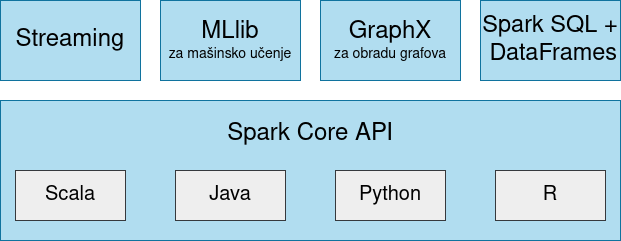
\includegraphics[width=1\textwidth]{pictures/spark_components.png}
  \caption{Компоненте Спарка}
  \label{fig:spark_kompot}
\end{figure}

Настао je 2009. године на универзитету Беркли у Калифорнији. Написан је у програмском језику Скала и конструисан је са идејом да користи концепте функционалног програмирања. Постао је део Апачи фондације 2013. године и од тада је доживео велики број промена. До сада, избачене су три верзије Апачи Спарка, редом, Спарк 1.0 (2013. године), Спарк 2.0 (2016. године) и Спарк 3.0 (2020. године).

\subsection{Архитектура}
\label{subsec:spark_arx}

Да бисмо користили Спарк на кластеру, прво је потребно да се прикачимо на њега коришћењем ресурс менаџера. Иако Спарк има свој лични ресурс менаџер, можемо користити и већ поменути Јарн или неки други. Након тога, можемо покретати Спарк апликације на кластеру.

Свака Спарк апликација се састоји из једног драјвер процеса (енг. \textit{driver process}) и једног или више егзекјутор процеса (енг. \textit{executor process}). Драјвер процес је срце Спарк апликације и задужен је за три ствари: одржавање информација о апликацији, реаговање на програм апликације и њен унос као и анализирање, распоређивање и планирање послова који се извршавају на егзекјуторима. 

Егзекјутори су ти који извршавају неки посао који им драјвер програм задаје. Сваки егзекјутор је задужен за две ствари: извршавање кода који му драјвер додељује и пријављивање стања извршавања тог кода драјверу. Једноставни приказ Спарк апликације је приказан на слици \ref{fig:spark_arhtt}. \cite{spark_guide}

\begin{figure}[!ht]
  \centering
  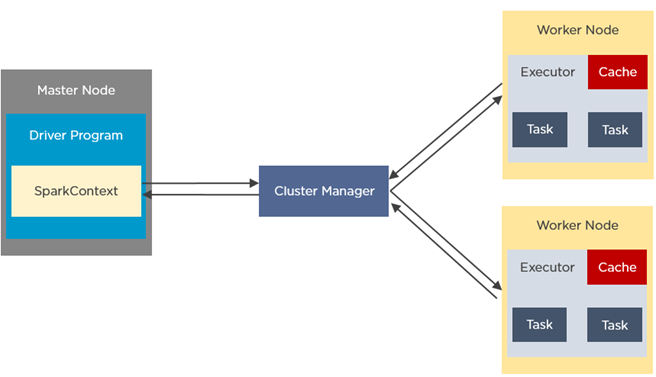
\includegraphics[width=1\textwidth]{pictures/spark_architecture.png}
  \caption{Архитектура Спарка}
  \label{fig:spark_arhtt}
\end{figure}

На приказаној слици се појављује концепт који није поменут до сада, а то је спарк контекст (енг. \textit{spark context}). Налази се унутар драјвера и његова улога је да дефинише конекцију ка кластеру. Поред тога, користи се за дефинисање спаркових апстракција које називамо РДД, о којима ће бити речи у наставку. 

Напоменимо да иста архитектура важи и када спарк покрећемо у локалном моду, на једној машини. Тада ће драјвер и егзекјутори и даље бити раздвојени процеси али ће радити на истој машини, а не на засебним. \cite{spark_guide}

\subsection{Партиције}
\label{subsec:spark_partic}

Да би егзекјутори могли паралелно да извршавају операције над подацима, Спарк их дели на делове које називамо партиције (енг. \textit{partitions}). Партиција је дакле један део колекције података који се налази на једној машини кластера. \cite{spark_guide}

Уколико су подаци партиционисани само једном партицијом сви ће се бити обрађени од стране једне машине у кластеру, независно од тога колико машина постоји. Слично, уколико смо креирали више партиција, али имамо само један егзекјутор, ниво паралелизма ће бити један због тога што постоји само једна машина која може да обради те податке. \cite{spark_guide}

\subsection{РДД}
\label{subsec:spark_rdd}

Основна јединица рада у Спарку се назива РДД (енг. \textit{RDD, resilient distributed dataset}) и све операције са подацима се извршавају преко ње. РДД је колекција елемената за које важи да су партиционисани по машинама кластера и да се над њима паралелно могу извршавати операције. \cite{spark_rdd} Дакле, један РДД се састоји од једне или више партиције падатака. \cite{spark_guide}

\begin{figure}[!ht]
  \centering
  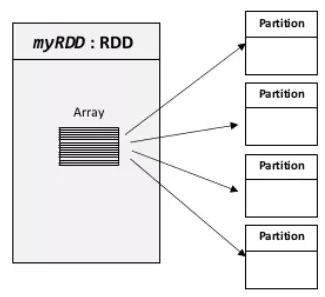
\includegraphics[width=0.5\textwidth]{pictures/spark_rdd.png}
  \caption{Спарк РДД}
  \label{fig:sprk_rdd}
\end{figure}

Постоји неколико начина преко којих можемо направити нови РДД:
\begin{itemize}
\item Читањем неког фајла који се налази на фајл систему (обично ХДФС)
\item Од неке колекција података програмског језика у коме користимо спарк. Тај процес дељења колекције у партиције називамо паралелизација
\item Од неког већ постојећег РДД
\item Кеширањем постојећег РДД
\end{itemize}

Данас се РДД апстракција не користи директно, већ постоје друге које су конструисане над РДД апстракцијом које су је потиснуле, па се РДД сматра застарелим.

\subsection{Трансформације}
\label{subsec:spark_transf}

Спарк је конструисан по принципима функционалног програмирања па су све његове структуре података имутабилне, што значи да се након њиховог креирања не могу мењати. Ако податке не можемо мењати, како их онда можемо обрађивати? Спарк то решава тако што свака промена над подацима у ствари креира потпуно нову струкуру података. На пример, уколико имамо један РДД и на неки начин желимо да променимо податке које он садржи, нећемо променити тај РДД, већ ћемо од њега направити нови који у себи садржи измењене податке. \cite{spark_guide}

Тај процес, где од једног РДД-ија применом неких наредби добијамо други, називамо трансформација (енг. \textit{transformation}). Пратећи функционалне концепте, трансформације немају никакве бочне ефекте, што значи да се од једног РДД-ија применом истих трансформација увек као резултат добија један исти РДД, независно од тога када се те трансформације примењују. РДД који трансформацијом настаје од другог РДД-ија називамо зависни РДД (енг. \textit{dependency}). \cite{spark_guide}

Постоје две различите врсте трансформација, уске (енг. \textit{narrow}) и широке (енг. \textit{wide}). За уске трансформације важи да једна партиција у оригиналном РДД доприноси настајању највише једне партиције у зависном РДД. Са друге стране, широке трансформације су такве где једна партиција почетног РДД учествује у конструисању више партиција зависног РДД, често свакој. Ово се другачије назива и мешање (енг. \textit{shuffle}) због тога што се врши размена партиција по кластеру. Јасније објашњење трансформација је приказано на слици \ref{fig:sprk_trnsf}. \cite{spark_guide}

\begin{figure}[!ht]
  \centering
  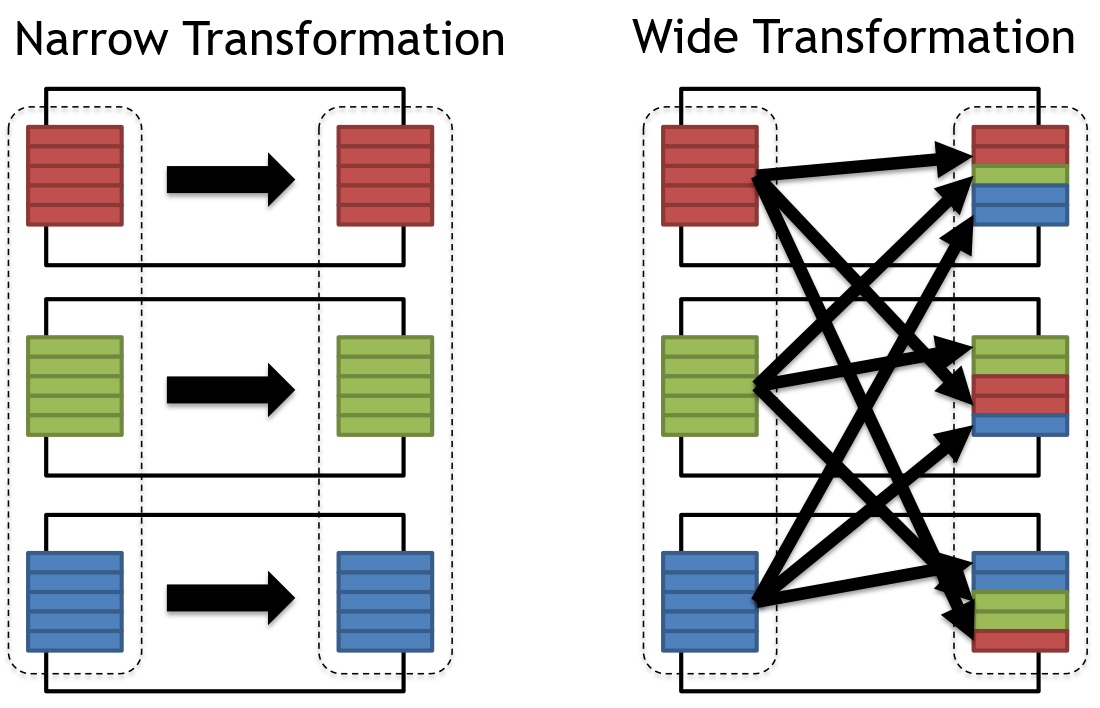
\includegraphics[width=1\textwidth]{pictures/spark_transformation_types.png}
  \caption{Приказ трансформацијa Спарка}
  \label{fig:sprk_trnsf}
\end{figure}

Постоји значајна разлика у перформансама узмеђу уских и широких трансформација. Код уских, спарк извршава операције у меморији, док код широких пише резултате на диск и распоређује их по меморији, што значајно успорава извршавање. \cite{spark_guide}

\subsection{Лења евалуација}
\label{subsec:spark_lazy_eval}

Лења евалуација значи да ће Спарк сачекати последњи тренутак да изврши дефинисане трансформације. Када имамо РДД и над њим дефинишемо неколико трансформација, оне неће бити одмах извршене, већ ће се од њих направити план трансформација који ће се извршити тек када се затражи њихов резултат. Разлог тога је ефикасност. Када Спарк зна које ће се све трансформације извршити над неком структуром података, може оптимизовати цео процес на такав начин да добијање резултата траје најкраће могуће. \cite{spark_guide}

\subsection{Врсте РДД трансформација}
\label{subsec:spark_transformation_types}

У овој секцији ћемо се упознати са неким трансформацијама које се најчешће користе. Вероватно најпознатија трансформација је \textit{map()} трансформација која за сваки елемент почетног скупа података производи нови, примењујући неку операцију на њега. Поред тог мапирања спарк нуди и флет мап \textit{FlatMap()} трансформацију, која за сваки елемент података производи нула, један или више елемената.

Још једна трансформација која се често користи је \textit{filter()} која за сваки елемент почетног скупа производи нула или један елемент новог скупа. Не врши никакве промене елемената, већ само од једног скупа елемената прави други скуп елемената од којих сваки задовољава неки услов.

Од широких трансформација су вероватно најпознатије редуковање по кључу \textit{reduceByKey()} и \textit{join()}. Обе раде са паровима кључ-вредност. Првом је улога да за сваки кључ сабере вредности са којима је упарен (слика \ref{fig:sprk_red_by_key}) док други на основу вредности кључа спаја два скупа у један, где ће у резултујућим подацима вредност кључа бити унија вредности кључа два скупа која учествују у спајању.

\begin{figure}[!ht]
  \centering
  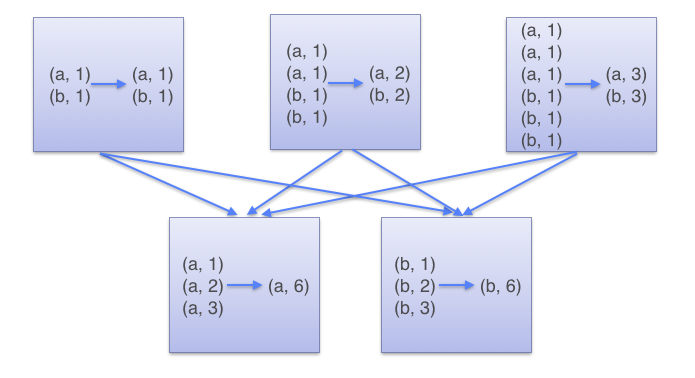
\includegraphics[width=1\textwidth]{pictures/spark_reduce_by_key.png}
  \caption{Редуковање по кључу}
  \label{fig:sprk_red_by_key}
\end{figure}

Поред ових трансформација постоје и \textit{union()}, \textit{intersect()}, \textit{sortByKey()}, \textit{groupByKey()} али и многе друге. \cite{spark_rdd}

\subsection{Акције}
\label{subsec:spark_akc}

Спарк акције користимо када желимо да затражимо резултат ланца трансформација. Дакле, тек када над нечим позовемо акцију заправо започињемо извршавање. Добијени резултат се враћа драјвер програму. \cite{spark_guide}

Постоје три врсте акција:
\begin{itemize}
\item акције које приказују резултат у конзоли
\item акције које исписују резултат у некакав излаз, на пример фајл
\item акције које пребацују податке у објекте неког програмског језика у коме користимо спарк
\end{itemize}

Неке од трансформација су \textit{count()}, \textit{take()}, \textit{saveAsTextFile()}, \textit{collect()} али постоје и друге. \cite{spark_rdd}

\subsection{Руковање грешкама у Спарку}
\label{subsec:spark_dags}

Нажалост, могуће је да се током извршавања догоде неки проблеми и да због тога изгубимо партицију. Уколико се то деси, Спарк је у могућности да реконструише изгубљене партиције уз помоћ механизма који се назива граф наследства (енг. \textit{lineage graph}). За сваки РДД, Спарк чува информације о томе од ког је РДД настао и које су трансформације примењене да бисмо добили тај РДД. Тај граф се може приказати сликом \ref{fig:sprk_ppln}.

\begin{figure}[!ht]
  \centering
  \includegraphics[width=1\textwidth]{pictures/spark_pipeline.png}
  \caption{Пример једног Спарк извршавања}
  \label{fig:sprk_ppln}
\end{figure}

Уз помоћ овог механизма Спарк зна од које партиције је настала свака од партиција и уколико нека партиција нестане, може је рекреирати. То ради тако што се креће кроз граф. Ако једна партиција није валидна, Спарк ће проверити партицију (или партиције) од којих је она настала. Уколико оне постоје, рекреираће невалидну партицију. У супротном, прегледаће рекурзивно партиције од којих је та партиција настала. И то ће радити све док не пронађе валидну партицију или не дође до партиције која је настала директним читањем из меморије. У том случају ће је прочитати поново. \cite{hadoop_learning}

Цео овај систем је поуздан из два разлога. Први је тај што трансформације немају бочне ефекте, па знамо да ћемо рекреирањем увек добити један исти РДД. Други је тај што се подаци чувају у ХДФС-у, који је сам по себи поуздан, па ако дођемо у ситуацију да морамо поново да рекреирамо цео ланац из почетка, знамо да ћемо прочитати непромењену вредност са диска.

\subsection{Кеширање}
\label{subsec:spark_persist}

Веома битна карактеристика Спарка је могућност да чува податке у меморији, односно да их кешира. Када се РДД кешира, свака машина у кластеру ће у својој меморији сачувати партиције које се на њој налазе и касније ће их користити у акцијама или трансформацијама које користе тај РДД. Овакав приступ знатно побољшава перформансе програма. \cite{spark_rdd}

РДД можемо кеширати коришћењем \textit{cache()} или \textit{persist()} метода. Када први пут тај РДД буде учествовао у некој акцији, сачуваће се у меморији и моћи ће да се користи у будућности. Кеширање је отпорно на грешке, тако да ако се једна од партиција изгуби, можемо је рекреирати из претходних трансформација. \cite{spark_rdd}

Постоје различити нивои кеширања у зависности од тога у којој меморији се чувају партиције. Уколико желимо да то буде меморија, можемо позвати \textit{cache()} метод али можемо и \textit{persist()} методу проследити вредност \textit{MEMORY\_ONLY}. 

Могуће је да у меморији нема места да би се РДД сачувао па због тога то можемо урадити и на диску. Тада прослеђујемо \textit{DISK\_ONLY}. Овај приступ се углавном не саветује из тог разлога што је често брже рекреирати цео ланац трансформација поново, него читати вредности са диска. Вредности \textit{MEMORY\_ONLY\_2} и \textit{DISC\_ONLY\_2} користимо када желимо да уз чување на тренутној машини извршимо репликацију на још једну машину. Поред тога, можемо бирати мешовити приступ (\textit{MEMORY\_AND\_DISC}). У том случају ће се РДД кеширати у меморији уколико има простора, а уколико не, чуваће се на диску. \cite{spark_rdd}

\subsection{Спарк Дата Фрејм}
\label{subsec:spark_df}

Дата фрејм је дистрибуирана колекција налик табели, са дефинисаним редовима и колонама. Свака колона мора имати исти број редова и сваки ред мора имати исти број колона, иако можемо користити недостајуће вредности. Поред тога, свака колона има један тип и тог типа морају бити све вредности које се налазе у редовима. \cite{spark_guide}

Сваки Спарк дата фрејм садржи метаподатке који описују имена колона и њихове типове. Те метаподатке називамо шема (енг. \textit{schema}). Шему можемо дефинисати мануелно али је и можемо закључити из података. \cite{spark_guide}

Спарк нуди велики број типова колона, који се мапирају у типове програмских језика преко којих користимо Спарк. Постоје једноставни типови попут целобројних и децималних бројева и ниски али постоје и сложени попут низова, мапа и датума. \cite{spark_guide}

\subsection{Трансформације и акције дата фрејма}
\label{subsec:spark_sql_ac_tr}

Све што важи за трансформације и акције које примењујемо над РДД, важи и за трансформације и акције које примењујемо над дата фрејмом. Трансформације немају бочни ефекат и лење су, тако да се извршавају тек када се над њима позове нека акција.

Једина разлика је та што РДД и дата фрејм другачије представљају податке па су им акције другачије. На пример, дата фрејм има акцију \textit{select(columns)} коју користимо да од једног дата фрејма добијемо други али са подскупом колона првог. Друга је \textit{filter(condition)} коју користимо да бисмо изабрали одређене редове једног дата фрејма и тако направили други. Ове две трансформације су идентичне редом \textit{SELECT} и \textit{WHERE} наредбама у програмском језику \textit{SQL}. Поред њих постоји и \textit{withColumn(name, expression)}, уз помоћ коje додајемо нову колону на постојећи дата фрејм. Наравно, постоји још велики број других. \cite{spark_guide}

Неке од акција које можемо применити на дата фрејм су на пример, \textit{collect()}, која нам омогућава да користимо податке унутар дата фрејма у програмском језику преко ког користимо Спарк и \textit{show()} коју користимо када хоћемо да испишемо дата фрејм на стандардни излаз. \cite{spark_guide}

\subsection{Разлика између дата фрејма и РДД}
\label{subsec:spark_df_vs_rdd}

Поставља се питање зашто бисмо користили један од ова два модела пре другог. РДД се користи за програмирање ниског нивоа и омогућава нам да директно вршимо операције над партицијама. Уколико желимо да користимо РДД за обраду података морамо бити веома пажљиви како пишемо код, коју трансформацију примењујемо и када, због тога што то може бити веома битно када су у питању перформансе. \cite{spark_guide}

Са друге стране, дата фрејм нема тих проблема. Све трансформације које напишемо над неким дата фрејмом пролазе кроз процес оптимизације тако да ћемо увек добити најоптимизованији могући код. Оптимизатор који је задужен за овај процес називамо Каталист (енг. \textit{Catalyst}). \cite{spark_guide}

Због тога, али и због једноставнијег интерфејса, дата фрејм је скоро потпуно потиснуо РДД из употребе.

\subsection{Планови извршавања}
\label{subsec:spark_exec_plans}

Процес извршавања дата фрејм кода изгледа овако:
\begin{enumerate}
\item Напишемо дата фрејм код
\item уколико је исправан, од њега се прави логички план
\item Спарк од логичког плана конструише физички план, успут примењујући оптимизације
\item Добијени физички план се пребацује у РДД и извршава се
\end{enumerate}

Дакле, након што се дата фрејм код прогласи исправним, од њега се конструише неразрешен логички план (енг. \textit{unresolved logical plan}) који представља апстрактне трансформације које треба извршити, али не садржи никакве изформације о томе над којим табелама или колонама треба извршити те трансформације. Те информације Спарк добија уз помоћ каталога (енг. \textit{catalog}) који садржи потребне информације. Резултат примене каталога на неразрешен логички план је логички план (енг. \textit{logical plan}). Након тога се тај план оптимизује од стране Каталиста, који оптимизује логички план тако што га анализира и примењује одређена правила на њега. Резултат је оптимизовани логички план (енг. \textit{optimized logical plan}). \cite{spark_guide}

Након што се оптимизовани логички план успешно креира, Спарк у односу на њега конструише неколико физичких планова (енг. \textit{physical plan}). Физички план дефинише како ће се логички план извршити на кластеру. Сви физички планови се након тога евалуирају и бира се онај који даје најбољи резултат. Тај физички план се онда преводи у РДД трансформације и ивршава на кластеру. \cite{spark_guide}

Цео процес је приказан на слици \ref{fig:sprk_ex_plns}.

\begin{figure}[!ht]
  \centering
  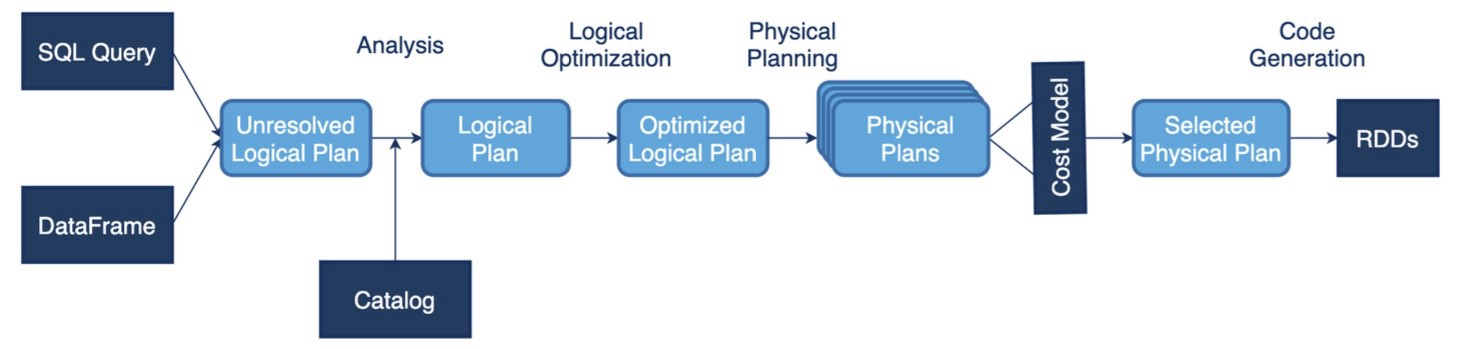
\includegraphics[width=1\textwidth]{pictures/spark_logical_plan.jpeg}
  \caption{Ток извршавања Спарк дата фрејма}
  \label{fig:sprk_ex_plns}
\end{figure}


\subsection{Остале компоненте Спарка}
\label{subsec:spark_components}

Поред поменутих компоненти које нам Спарк нуди постоје и многе друге али се њима нећемо бавити у овом раду због тога што су ван опсега. Спарк, поред РДД и дата фрејм интерфејса нуди још два, дата сет (енг. \textit{spark dataset}) и спарк сикуел (енг. \textit{spark sql}). Веома су слични дата фрејму и пролазе кроз исти процес компилације али ипак постоје неке мање разлике. \cite{spark_guide} 

Спарк сикуел се користи за извршавање упита над кластером. Једина разлика је у томе што се грешке које настају овим методом појављују док се код извршава, а не у компилацији. \cite{spark_guide}

Разлика између дата сета и дата фрејма је у типовима. Наиме, разлика је у томе што што се типови колона дата фрејма проверавају са онима у шеми у току извршавања програма, док се код дата сета то дешава за време компилације. Такође, разлика је у томе што је дата сет доступан само у ЈВМ (енг. \textit{JVM}) базираним језицима, скали и јави, док у другима не постоји. \cite{spark_guide}

Поред тога Спарк омогућава конструисање модела машинског учења над подацима преко библиотеке која се назива \textit{Spark ML lib}. Она се може користити за препроцесирање, тренирање модела и прављење предвиђања. \cite{spark_guide}

Спарк нуди и операције над стримовима (токовима) података. Можемо се закачити за некакав ток и над њим можемо примењивати исте операције које смо поменули у претходним секцијама овог рада (на пример у дата фрејм секцији). Спарк стриминг омогућава преплату на токове података који настају из неког веб сокета (енг. \textit{socket}), од неке групе фајлова, или које производи Апачи Кафка. \cite{spark_streaming}

За сам крај, поменимо да Спарк поред свега тога има библиотеку за рад са графовима, \textit{graphX} али се данас за обраду графова често користе нека друга решења. \cite{spark_guide}

% ако хоћеш да причаш о каталисту можеш наћи овде https://databricks.com/blog/2015/04/13/deep-dive-into-spark-sqls-catalyst-optimizer.html

\chapter{Семантички веб}
\label{chp:sem_veb}

Веб је током свог постојања константно еволуирао. Разликују се три веће етапе које су назване по редним бројевима, Веб 1.0, Веб 2.0 и Веб 3.0.

\section{Веб 1.0}
\label{sec:sem_veb_veb_1}

Ова верзија представља прву фазу еволуције веба. Настао је у последњим деценијама 20. века и трајао је до средине прве деценије 21. Карактерише га скуп статичког садржаја који је повезан преко веза названих \textit{hyperlik}.

Уз помоћ њега су представљане само информације које су се приказивале корисницима. Још увек није постојао језик за улепшавање страница, \textit{CSS} и није било динамичких линкова, логовања корисника и остављања коментара.

%Веб страница Свемирског баскета (енг. \textit{Space Jam}), популарног филма из 90-тих нам даје увид у то како је изгледала једна страница тада, пошто је непромењена од тренутка када је направљена, 1996. године. Можемо је пронаћи на адреси https://www.spacejam.com/1996/.

%\begin{figure}[!ht]
%  \centering
%  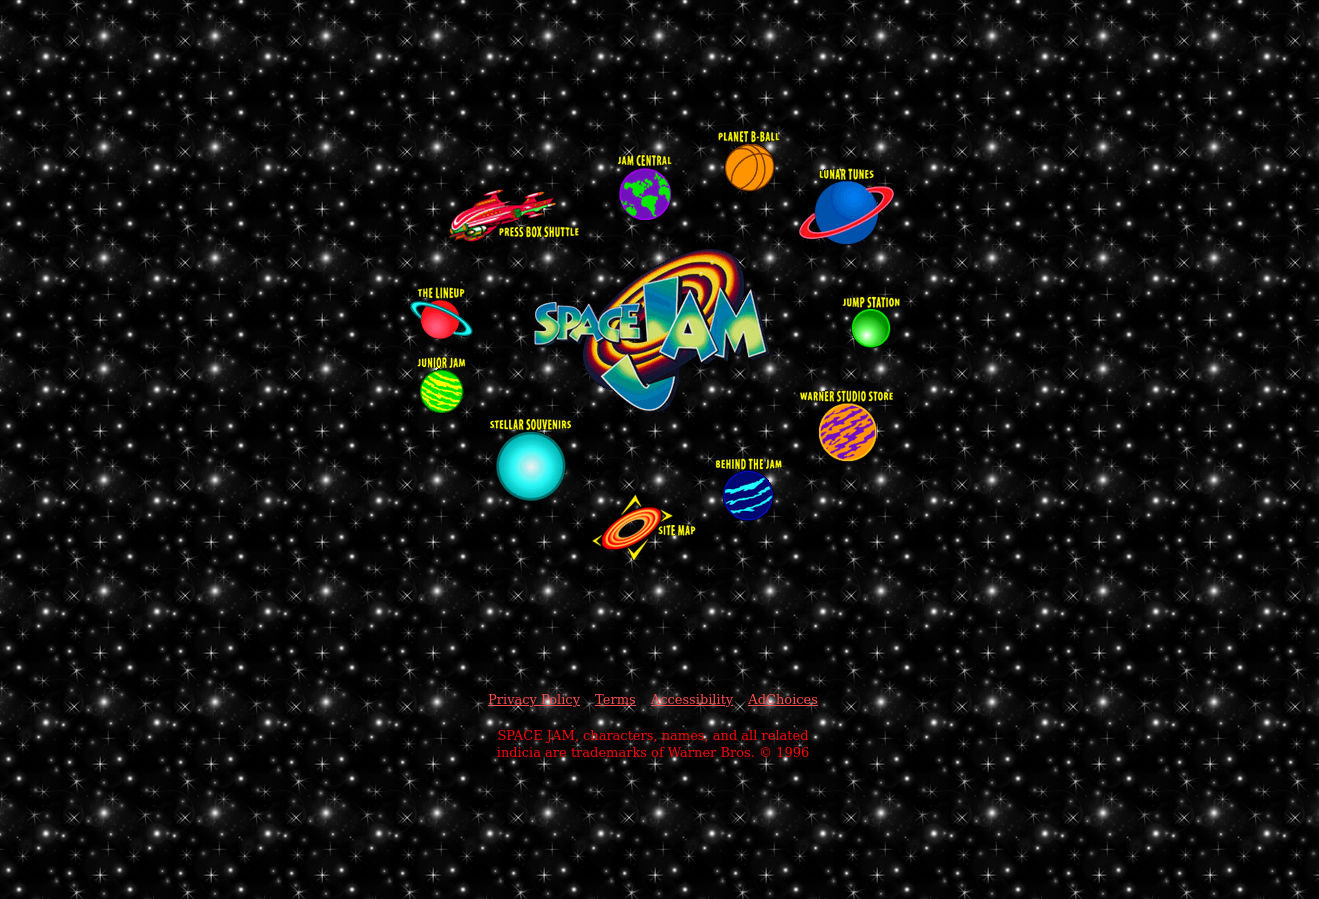
\includegraphics[width=1\textwidth]{pictures/space_jam.png}
%  \caption{Веб страница Свемирског баскета}
%  \label{fig:sem_veb_space_jam}
%\end{figure}

\section{Веб 2.0}
\label{sec:sem_veb_veb_2}

Друга фаза је почела одмах након прве и траје и дан данас. Акценат је стављен на садржај генерисан од стране корисника, једноставно коришћење као и на размени информација. У овој фази је, преко програмских језика који се извршавају на серверској страни, омогућен рад разних апликација попут Амазона (енг. \textit{Amazon}), Ју Тјуба (енг. \textit{YouTube}) и Фејсбука (енг. \textit{Facebook}). Све то је омогућило корисницима да на једноставан начин деле и размењују своја мишљења и искуства.

%\begin{figure}[!ht]
%  \centering
%  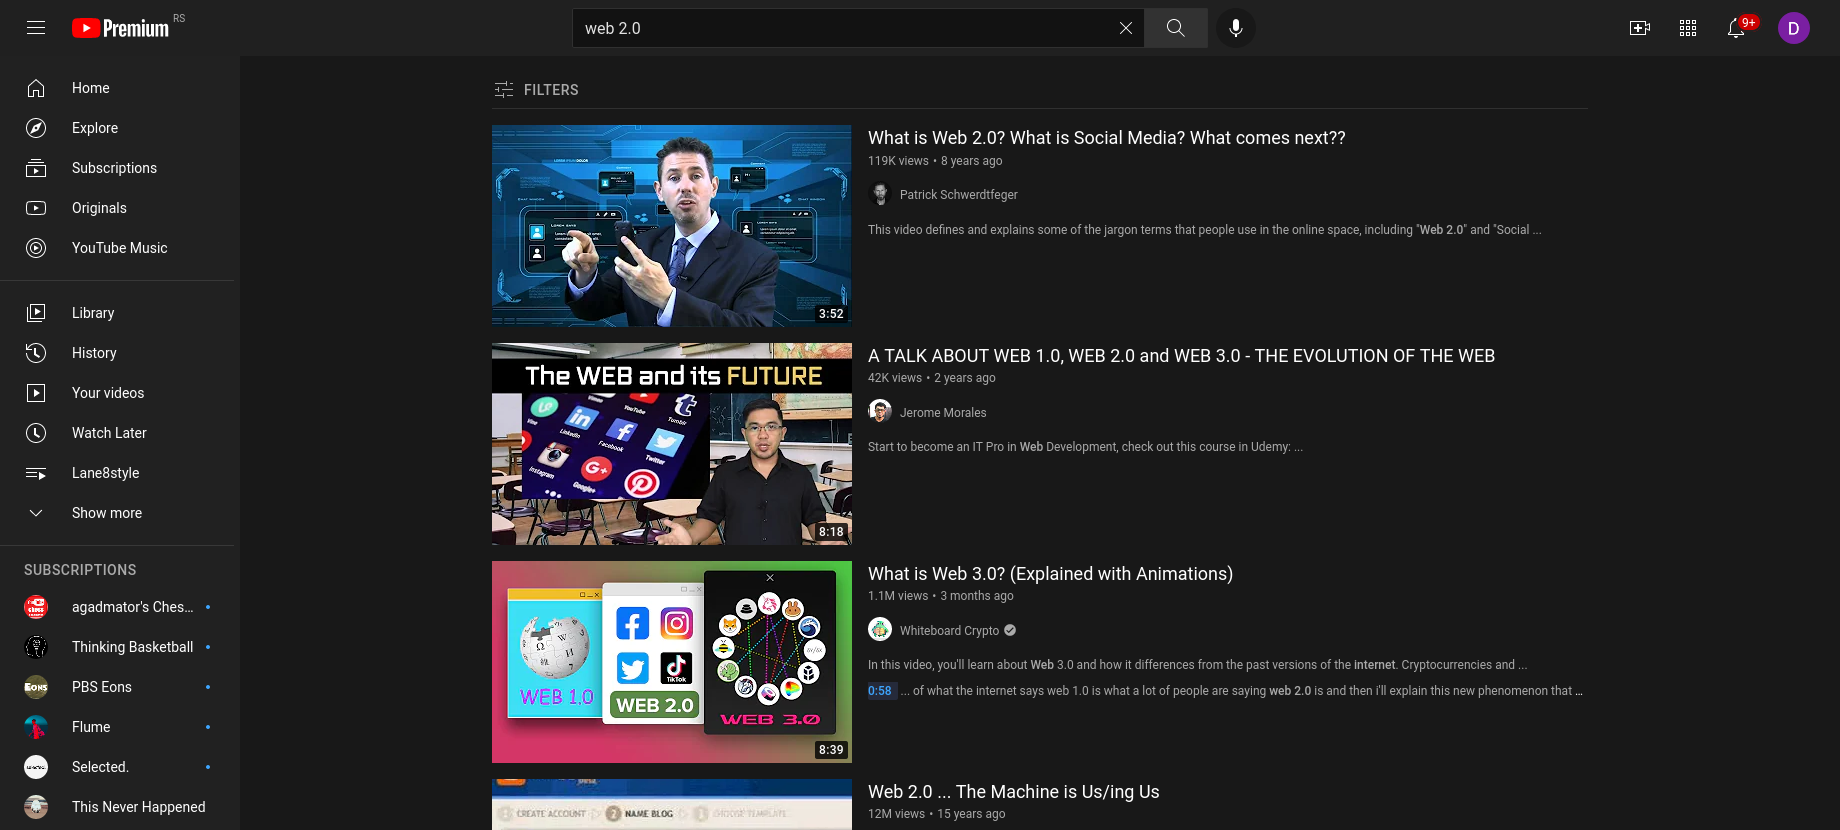
\includegraphics[width=1\textwidth]{pictures/youtube_page.png}
%  \caption{YouTube веб страница}
%  \label{fig:sem_veb_you_tube_page}
%\end{figure}

Међутим, Веб 2.0 има једну велику ману, а то је да се сви подаци, које поменуте апликације сакупљају, складиште на приватним серверима које контролишу корпорације. Велики број њих користи те податке да би кориснике што дуже задржалo на својим сервисима. Такође, у неколико инстанци су ти подаци продавани некој другој страни, у циљу једноставне зараде. Због овога се може рећи да су корисници постали производ друге фазе веба.

\section{Веб 3.0}
\label{sec:sem_veb_veb_3}

Циљ треће верзије веба је да се ослободи централизације присутне у вебу 2.0 и направи децентрализован али сигуран интернет где би људи могли да размењују информације без посредника, ког тренутно представља корпорација чије услуге ти корисници користе.

Последица децентрализације је та да апликације више неће бити покретане преко огромних, приватних, база података и сервера, већ ће се прећи на технологије као што су блокчеин (енг. \textit{blockchain}) и мреже равноправних корисника (енг. \textit{peer-to-peer}).

Идеја је да у самом срцу веба 3.0 стоји семантички веб, чија би улога била да повеже постојеће податке и информације које се налазе на интернету, и направи их таквим да њихов садржај и контекст могу разумети машине.

\begin{figure}[!ht]
  \centering
  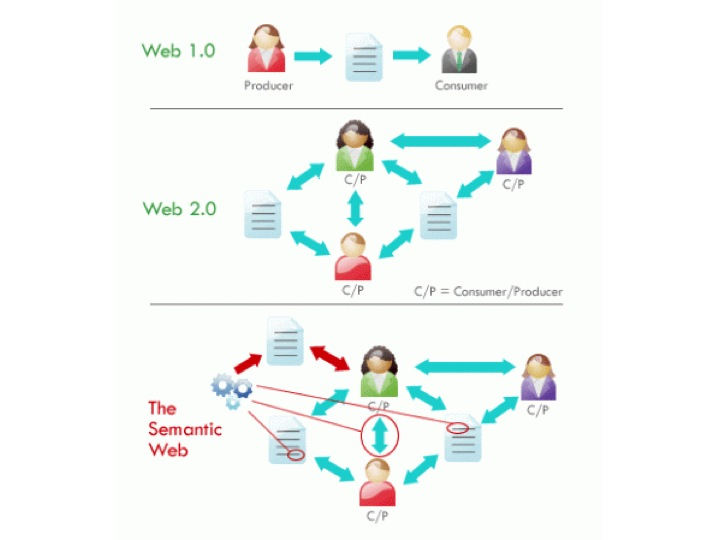
\includegraphics[width=1\textwidth]{pictures/webs_vrs.jpg}
  \caption{Фазе Веба}
  \label{fig:sem_veb_versions}
\end{figure}

Ова верзија Веба је још увек у развоју, са огромним простором за даље истраживање. Међутим, како је сама архитектура доста комплекснија од архитектуре Веба 2.0, није сигурно да ли ће заживети и ако да, када. Али оно што је сигурно је да идеја о дељеним подацима и децентализованом вебу и даље постоји и велики број људи је развија и унапређује.

%Један од примера веб 3.0 апликације је \textit{odysee} направљена за дељење видео снимака и сматра се децентрализованом алтернативом \textit{YouTube}-a. Ова апликација користи \textit{LBRY} протокол \cite{lbry} који је базиран на блокчеин технологији и користи се за дељење фајлова и плаћање. \cite{odysee_article}

%Тим који стоји иза ове апликације сматра да је \textit{YouTube} превише стриктан у томе који садржај бира да промовише и блокира. \textit{Odysee} je настала са идејом слободе говора и направљена је тако да је свако може користити да промовише своје погледе на свет. \cite{odysee_article}

%Идеја иза веба 3.0 је таква да интернет више не контролишу компаније које поседију сервере, већ да се та контрола пребаци на кориснике. Самим тим, информације о корисницима се више неће налазити на приватним серверима, већ ће бити пребачене код самих корисника, уз помоћ блокчеин технологије.  \cite{coinbase_web3}

%То доводи до огрмоних промена у томе како веб функционише. Архитектура веба 2.0 је једноставна. Састоји се од клијента, који је обично представљен интернет претраживачем или неком апликацијом, који комуницирају са серверима и од њих добијају информације уз помоћ којих функционишу. Ентитет који контролише сервере, контролише и који корисници могу да им приступају као и шта они могу да виде, па стога, један корисник може имати привилегован статус у односу на другог. Поред тога, чува информације о поменутим корисницима и о томе шта они на тим серверима поседују. \cite{coinbase_web3}

%У вебу 3.0, апликацијама је дозвољено да чувају садржај на јавно доступном блокчеину. Дакле, тај садржај постаје доступан свима. Такође, дозвољава корисницима директну контролу над тим садржајем. Идеја је да не постоји потреба за корисничким налозима или привилегованим АПИ (енг. \textit{API}) кључевима, већ да свако може да приступи свему. 

%Веб 3.0 то омогућава уз помоћ употребе крипто новчаника (енг. \textit{crypto wallet}), уз помоћ ког наша апликација шаље трансакције на блокчеин, и блокчеин чворова (енг. \textit{blockchain node}), чија је улога да надгледају и регистрију трансакције које се дешавају на блокчеину. \cite{coinbase_web3}

%Када крипто новчаник жели да пошаље неку трансакцију на блокчеин или када од њега захтева некакве информације, комуницираће са блокчеин чворовима. Преко тога је нашој апликацији омогућено да комунуцира са блокчеином и на тај начин она сакупља информације које су јој потребне да би правилно функционисала. Овај однос подсећа на однос који данашње апликације имају са својим приватним серверима. \cite{coinbase_web3}

%Поређење архитекура између две верзије веба је приказано на слици \ref{fig:sem_veb_veb3_arh}.

% https://www.coinbase.com/learn/crypto-basics/what-is-a-crypto-wallet

%\begin{figure}[!ht]
%  \centering
%  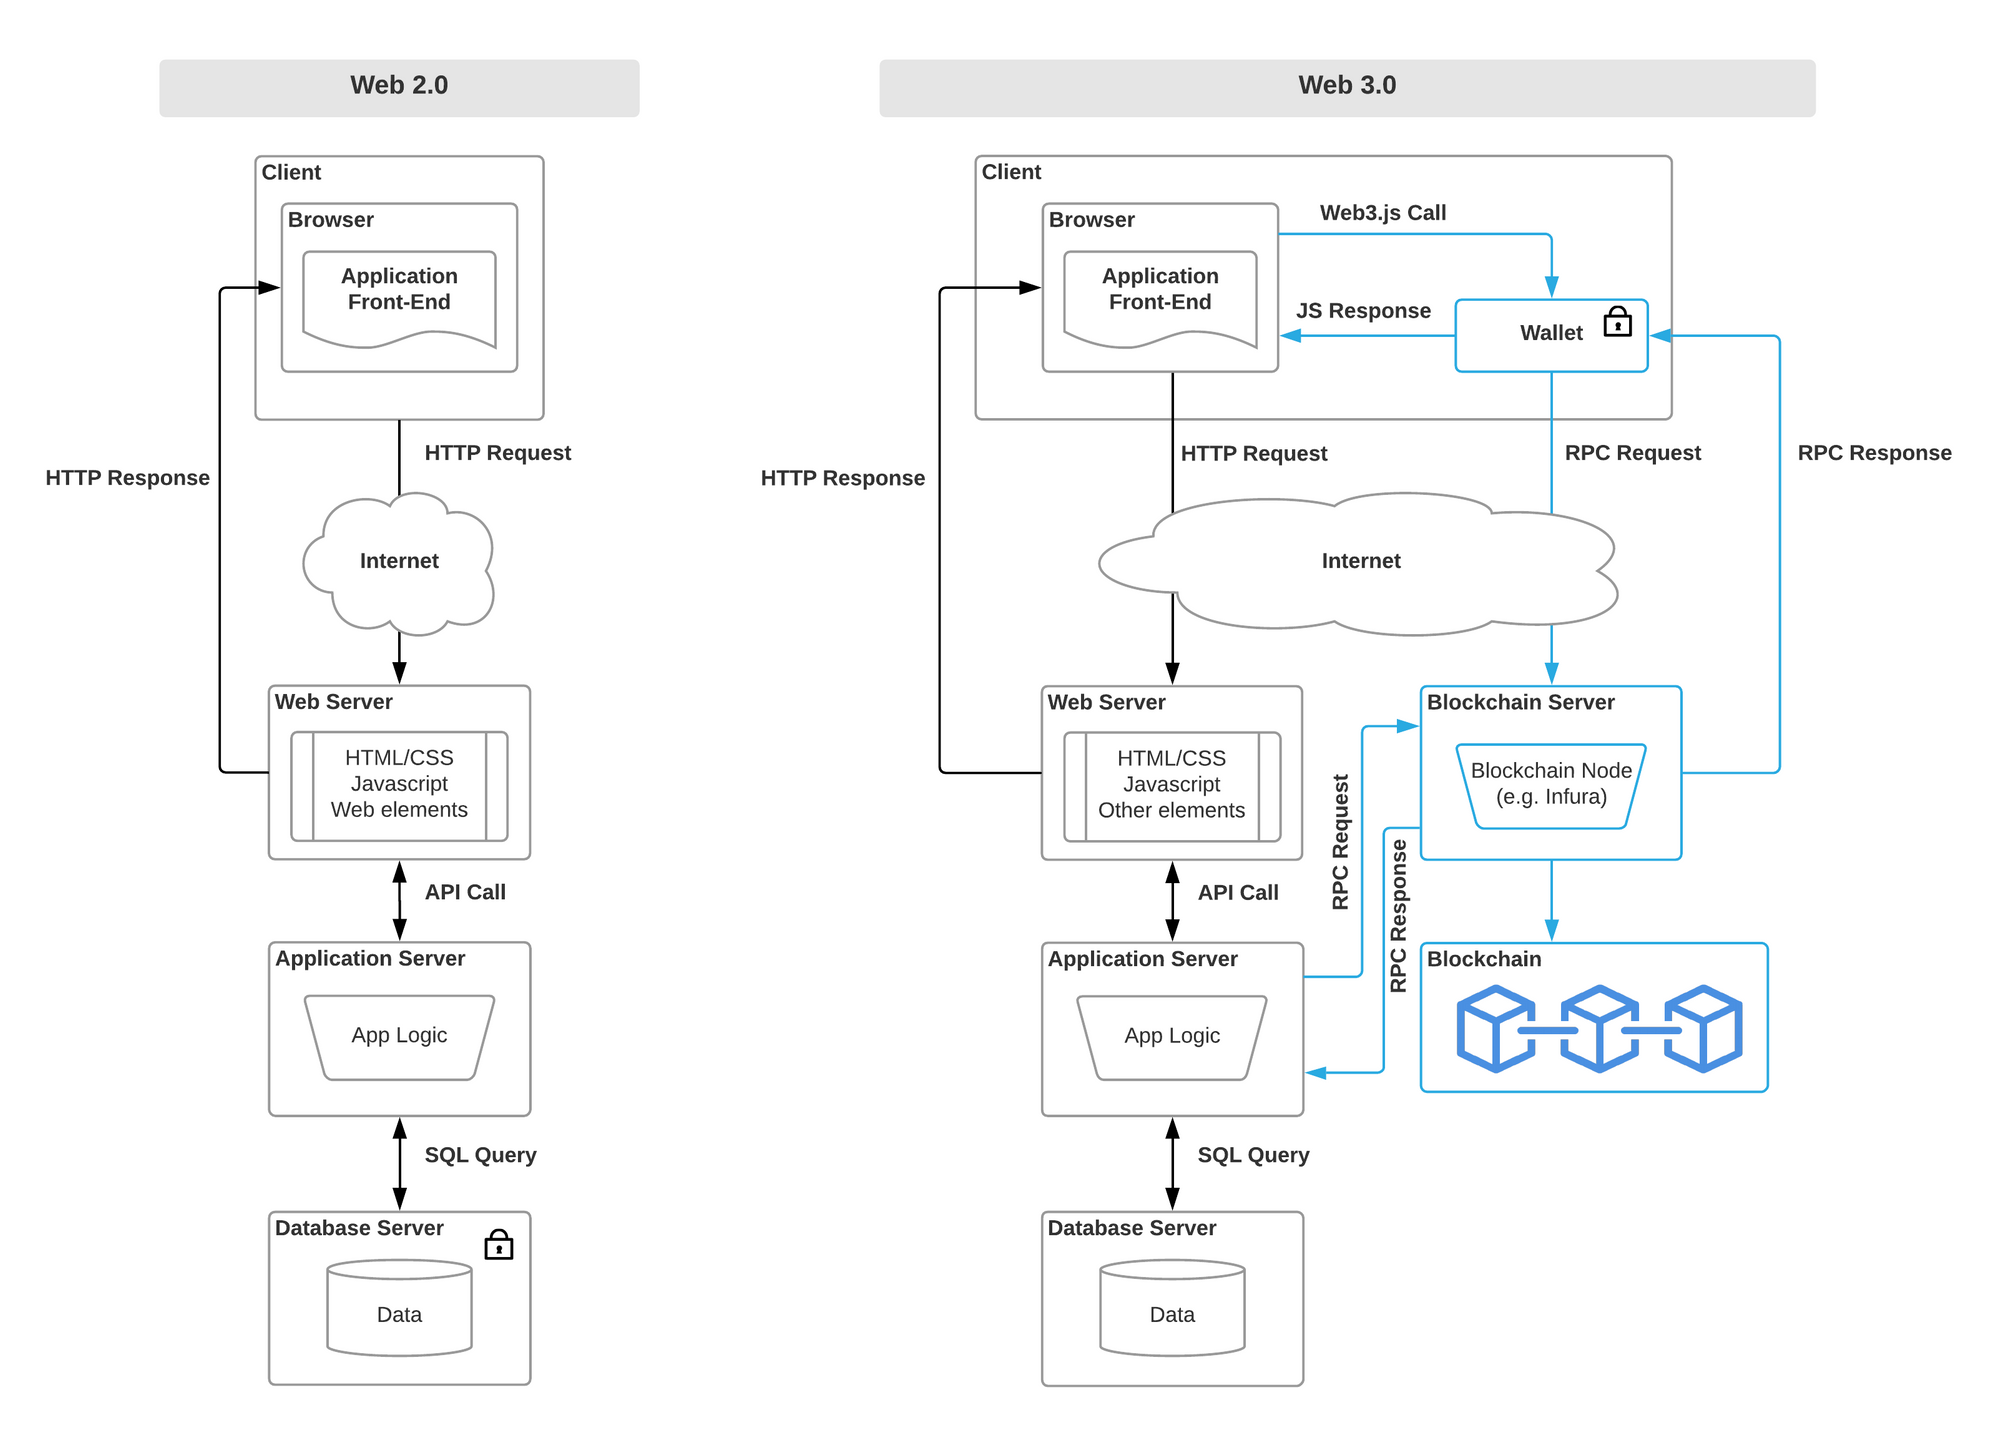
\includegraphics[width=1\textwidth]{pictures/veb3_arh.png}
%  \caption{Једноставан приказ архитектура веба 2.0 и веба 3.0}
%  \label{fig:sem_veb_veb3_arh}
%\end{figure}

%Наравно, веб 3.0 доноси и неколико проблема. Прво, тренутне машине које се користе за рударење криптовалута и праћење трансакција конзумирају огромне количине енергије, па ће стога њена потрошња бити велики проблем који се мора решити пре него што веб 3.0 постане стварност.

%Такође, сви подаци ће се и даље налазити на серверима али ти сервери неће бити у приватном власништву великих корпорација. То доноси неколико питања. На пример, ко је власник тих сервера? Ко плаћа нихово одржавање? Ко има информације о нашим налозима, попут шифри које користимо и других личних података? Дакле, неко ће ипак бити власник наших података, с тим што се поставља питање, ко тачно?

% https://www.stephendiehl.com/blog/web3-bullshit.html

%Ова верзија веба је још увек нова, са огромним простором за даље истраживање али се због свега наведеног није сигурно да ли ће икада заживети, и ако да, када? Оно што је сигурно да идеја о дељеним подацима и децентализованом вебу и даље постоји и велики број људи је развија и унапређује. У самом средишту дељења података се налази семантички веб.

\section{Семантички веб}
\label{sec:semantic_veb_main}

Семантички веб је надоградња садашњег веба, \textit{WWW}-а, који омогућава рачунарима да, на интелигентан начин, претражују и обрађују податке са веба. Интелигентно у овом случају значи да ће рачунари бити способни да закључе шта подаци представљају људима који их користе. Пошто до сада није конструисан ниједан систем вештачке интелигенције који може потпуно да опонаша човека, то се може постићи само ако се значење, то јест семантика, ресурса на вебу експлицитно представи рачунарима у формату у којем их они могу обрадити. \cite{semantic}

Да би се ово постигло, није довољно само складиштити податке у језику који машине разумеју, на пример у \textit{HTML} формату, већ је неопходно да се уз те податке додају и информације о семантици која јасно говори које закључке треба из њих извући. Међутим, тако нешто је врло вероватно немогуће извести због тога што је чак и људима тешко да се договоре око значења садржаја одређених страница на вебу, па је стога још теже формализовати тај садржај на такав начин да буде значајан машинама. \cite{semantic}

%Дакле, семантички веб заправо има намену да омогући машинама приступ већем броју информација, којима је до сада приступао само човек, у на тај начин доведе до смањења потрошње времена корисника интернета.
%То значи да семантички веб заправо има другу намену, а то је омогући машинама приступ  већем броју информација којима тренутно приступа човек, што доводи до смањења потрошње времена. То значи да семантички веб заправо није екстензија данашњег веба, већ некакав идеал ка коме веб временом еволуира. \cite{semantic}

Да би семантички веб функционисао, на неки начин се људско знање мора изразити неким формалним језиком. Тај проблем се може решити моделовањем. Један од језика који се користи у семантичком вебу је \textit{OWL 2} и настао је под утицајем коришћења моделовања у биологији. На који начин ће знање бити моделовано зависи од тога за шта ће конструисан модел бити коришћен. Код семантичког веба, идеја је да компјутерски програми закључују на основу датих информација на такав начин да узимају у обзир резоновање и формалну репрезентацију знања. \cite{semantic}

Дакле, развој семантичког веба се заснива на припајању моделовања знања и аутоматског закључивања вебу. Исто тако, на овај начин се веб апликације уводе у домен формалног моделовања и репрезентације знања. 

Иако су раније постојали примери стандардизације саме формалне репрезентације знања, семантички веб је допринео њеној важности и употребљивости. Велика већина релевантних покушаја стандардизације је спроведена од стране \textit{WWW} Конзорцијума, познатијег као \textit{W3C}. \cite{semantic}

%Исто тако, сам Веб у друге дисциплине уводи појам дистрибуираних али повезаних информација. Веб ставља акценат на важност јасно дефинисаних, стандардизованих језика који се користе за размену података између различитих јединица. 

\subsubsection{Историјат}
\label{subsubsec:semantic_timeline}

Идеја додељивања семантике вебу није нова и постојала је још у самом зачећу веба. Први покушаји су забележени код типизираних линкова (енг. \textit{typed links}) чија је улога била да, поред тога што су представљали референцу ка другом документу, садрже и неке информације о томе шта заправо тај линк представља. \cite{semantic}

Семантички веб је добио већу пажњу јавности 2001. године, када је Тим Бернерс Ли (енг. \textit{Tim Berners-Lee}) објавио чланак назван \textit{Семантички веб} у којем су представљене идеје о томе како би семантички веб функционисао. До данас је \textit{W3C}, чији је Тим Бернерс Ли члан, објавио неколико технологија међу којима су \textit{RDF, Resоurce Description Framework}, \textit{OWL, Web Ontology Language} и језик за упите \textit{SPARKQL}, али и многе друге. \cite{semantic}

Поред тога су забележени и покушаји у томе да се у \textit{HTML} документе, преко вредности атрибута, доделе неки семантички подаци једном веб документу. Те вредности се називају микроформати (енг. \textit{microformats}) и користе се за решавање проблема у специфичним доменима апликација, на пример, приликом енкодирања личних података. \cite{semantic}

Једноставан пример микроформата је \textit{HTML} атрибут \textit{rel} који се користи да би се назначило шта се налази на линку коме тај атрибут је додељен. У следећем примеру се користи да би се нагласило да се на приложеном линку налази лиценца.

\begin{lstlisting}[language=HTML]
<small>This article is licensed under a 
  <a rel="license" href="http://creativecommons.org/licenses/by-nc-sa/2.0/">
  Creative Commons Attribution Non-commercial Share-alike 
  (By-<abbr>NC</abbr>-<abbr>SA</abbr>) license</a>.
</small>
\end{lstlisting}

Количина семантичких података која је доступна на вебу се повећава из године у годину и подаци су постали међусобно повезани. Ово се дешава због тога што идентификатори који се користе у језицима семантичког веба прате исте принципе као и адресе класичног веба. Стога, име једног објекта семантичког веба се може интерпретирати као веб адреса. То доводи до појаве повезаних података (енг. \textit{linked data}) која се односи на семантичке податке чији су идентификатори заправо показивачи ка веб адресама на којима се може пронаћи више информација о објекту. \cite{semantic}

Због тога се користи термин \textit{веб података}, који описује семантички веб као покушај који се примарно фокусира на размену података. 

\subsection{RDF језик}
\label{subsec:semantic_rdf}

Механизам за описивање ресурса (енг. \textit{resource description framework}) или скраћено \textit{RDF} је формални језик за описивање структуираних информација. Поента овог језика је да омогући апликацијама да размењују податке на вебу задржавајући њихово оригинално значење. За разлику од језика као што су \textit{HTML} и \textit{XML}, циљ није приказати документе у правилном формату већ омогућити обраду информација које они садрже. Због свега наведеног \textit{RDF} се често сматра основом за развој семантичког веба. \cite{semantic}

Дакле, улога \textit{RDF}-а није да описује структуру докумената, већ да опише однос између неких објеката. Данас је овај формат веома распростањен и готово сваки виши програмски језик поседује библиотеке помоћу којих се могу извршавати разне операције над њим. \cite{semantic}
 
\textit{RDF} документ је описан усмереним графом, односно скупом чворова који су повезани усмереним гранама. Сваки чвор и свака грана имају засебан идентификатор. Структура графа је изабрана баш из тог разлога да би се изразио однос између објеката, а не њихова хијерархија. На пример, на слици \ref{fig:semantic_rdf_graph_example} се примећује да је однос између приказаних елемената, курса и студената, информација која нема јасну хијерахију. \textit{RDF} користи такав однос као основну јединицу информације. Штавише, велики број таквих односа производи графове. \cite{semantic}

\begin{figure}[!ht]
  \centering
  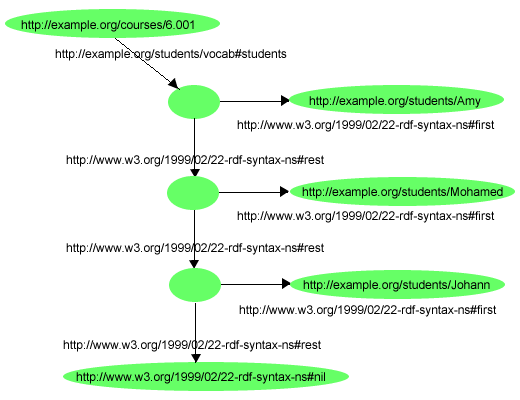
\includegraphics[width=0.8\textwidth]{pictures/rdf_graph_example.png}
  \caption{Пример РДФ графа}
  \label{fig:semantic_rdf_graph_example}
\end{figure}

Други разлог због кога је \textit{RDF} представљен графом је чињеница да му је улога да служи као описни језик података веба и других мрежа. Иформације у овим срединама се складиште и обрађују дистрибуирано па је стога битно комбиновати \textit{RDF} податке на једноставан начин. На пример, граф који је репрезентација једних података се лако може повезати са графом који представља нешто друго, једноставним повезивањем. Ако претпоставимо да поред графа на слици \ref{fig:semantic_rdf_graph_example} постоји, на пример, још један граф који описује студенте, лако се може закључити да се они једноставно могу повезати и користити заједно. \cite{semantic}

Додељивање имена \textit{RDF} документима може произвести проблеме. Наиме, именовање не мора бити униформно. На пример, могуће је да два документа садрже информације о истој теми, али да су им идентификатори потпуно различити. Такође, могуће је и да је једном истом ресурсу додељено неколико различитих имена или да се исти идентификатори користе за различите појмове.

Да би се тај проблем избегао \textit{RDF} користи униформни индикатор ресурса (енг. \textit{uniform resource identificator, URI}) као имена, у циљу разликовања ресурса. Напоменимо да је \textit{URI} генерализација \textit{URL} адреса које се користе за приступ документима на интернету. Како је сваки \textit{URL} валидан \textit{URI}, може се користити као идентификатор унутар \textit{RDF} докумената. У великом броју апликација циљ није разменити информације о веб страницама већ о великом броју објеката као што су на пример студенти, књиге, места, догађаји и тако даље. Таквим објектима се не може приступити на интернету па се њихов \textit{URI} користи ускључиво за идентификацију. Напоменимо и то да се \textit{URI} адресе које нису \textit{URL} називају \textit{URN}. \cite{semantic}

Због идентификације, чворовима и гранама унутар \textit{RDF} графа се додељује \textit{URI} као име, што можемо приметити и на већ приложеном примеру (слика \ref{fig:semantic_rdf_graph_example}). Ово правило има два изузетка. Први је тај да је ипак могуће доделити име које није \textit{URI}, а други је да је могуће не доделити име и оставити га празним, али се таквим случајевима нећемо бавити. \cite{semantic}

Иако \textit{URI} представљају имена, њихово значење је подложно интерпретацији па другачији алати могу на другачији начин да посматрају њихово значење. Због тога је уведен још један појам, литерал, који представља вредности унутар \textit{RDF}-а. Увек су записани ниском уз коју је припојен и њен тип. На пример, ниска \textit{"123"} може бити целобројног типа што би значило да представља број \textit{123}. За разлику од \textit{URI}-ја, литерали увек имају једно значење. У графу се представљају правоугаоним чворвима (слика \ref{fig:sem_rdf_graph_2})). \cite{semantic}

\begin{figure}[!ht]
  \centering
  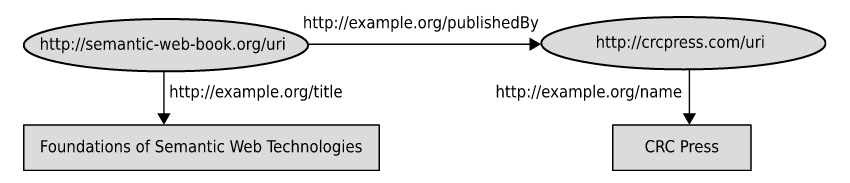
\includegraphics[width=0.8\textwidth]{pictures/rdf_graph_example_2.png}
  \caption{Пример РДФ графа са литералима}
  \label{fig:semantic_rdf_graph_2}
\end{figure}

\subsubsection{Репрезентација}
\label{subsubsec:semantic_rdf_representation}

Како су \textit{RDF} графови ретки, представљају се скупом грана које се у њему налазе. Једна грана је представљена вредношћу чворова, као и њеном ознаком. Чворове називамо субјекат и објекат, док се ознака назива предикатом. Тројка субјекат-предикат-објекат се другачије назива и \textit{RDF} тројком. Сваки члан тројке може бити некакав \textit{URI} али може бити и литерал. \cite{semantic}

Један од формата који се користе за репрезентовање \textit{RDF} графа је корњача (енг. \textit{turtle}) нотација. У овој нотацији се граф са слике \ref{fig:semantic_rdf_graph_2} приказује на следећи начин:

\begin{lstlisting}[language=XML]
<http://semantic-web-book.org/uri> <http://example.org/publishedBy> <http://crcpress.com/uri> .
	
<http://semantic-web-book.org/uri> <http://example.org/title> "Foundations of Semantic Web Technologies" .

<http://crcpress.com/uri> <http://example.org/name> "CRC Press" 
\end{lstlisting}

Међутим, овај запис, тачније \textit{URI} који му припадају, се може скратити увођењем префикса који означавају именска поља која представљају фамилију \textit{URI} адреса. Уз помоћ њих се исти запис може записати доста једноставније:

\begin{lstlisting}[language=XML]
@prefix book: <http://semantic-web-book.org/> .
@prefix ex: <http://example.org/> .
@prefix crc: <http://crcpress.com/> .

book:uri ex:publishedBy crc:uri .
book:uri ex:title "Foundations of Semantic Web Technologies" .
crc:uri ex:name "CRC Press" .
\end{lstlisting}

Поред корњача нотације, чест начин репрезентовања \textit{RDF} структуре је уз помоћ \textit{XML} формата. Разлог томе је што је тај формат читљив и људима и машинама, али и тај што скоро сваки програмиски језик поседује алате за обраду тог формата. Приказ једноставног \textit{RDF} графа са слике \ref{fig:semantic_rdf_graph_2} у \textit{XML} формату се може наћи у наставку:

\begin{lstlisting}[language=XML]
?xml version="1.0" encoding="utf-8"?>
<rdf:RDF xmlns:rdf="http://www.w3.org/1999/02/22-rdf-syntax-ns#"xmlns:ex ="http:/example.org/">
  <rdf:Description rdf:about="http://semantic-web-book.org/uri">
    <ex:publishedBy>
      <rdf:Description rdf:about="http://crcpress.com/uri">
      </rdf:Description>
    </ex:publishedBy>
  </rdf:Description>
</rdf:RDF>
\end{lstlisting}

%РДФ шема, страна 46 у књизи. можда то да додаш (\textit{RDF})

%\textbf{Chapter 7
%Query Languages
%In previous chapters, we learned about a number of possibilities for specifying
%information in a machine-readable way. RDF allows us to structure and relate
%pieces of information, and RDFS and OWL introduced further expressive
%means for describing more complex logical relations. The latter was further
%extended by means of logical rules that could be combined with OWL. For
%each of those description languages, we also introduced a notion of logical
%entailment: RDF(S) documents may entail other documents (Chapter 3),
%and OWL knowledge bases – possibly augmented with rules – can imply new
%axioms (Chapters 4, 5, 6)}


\subsection{OWL}
\label{subsec:semantic_owl}

\textit{OWL}, скраћено од \textit{Web Ontology Language}, је језик семантичког веба који се користи за представљање комплексног знања о стварима, њиховим групама или њиховим релацијама. Комплексно знање у овом контексту су инфомације које се не могу изразити преко \textit{RDF} формата. Овај језик спада у групу логичких језика, па се знање које изражава може користити унутар компјутерских програма. \textit{OWL} документ се назива онтологијом и могуће га је поставити на интернет, одакле га могу реферисати неке друге \textit{OWL} онтолигије. \cite{semantic}

Тренутна верзија овог језика је \textit{OWL 2}. 

%https://www.w3.org/2001/sw/wiki/OWL

\subsection{SPARQL}
\label{subsec:semantic_query}

Иако се информације из претходно поменутих \textit{RDF} и \textit{OWL} формата могу сазнати њиховом обрадом, то често у пракси није довољно. Због тога су настали упитни језици, чија је улога извлачење потребних информација из разних структура података семантичког веба. Упитни језик за \textit{RDF} је назван \textit{SPARKQL}. \cite{semantic}

Спаркл, или \textit{SPARQL}, \textit{SPARQL protocol and RDF query language}, је стандард за упите информација \textit{RDF} формата као и за представљање добијених резултата. Иако је синтакса овог језика веома слична синтакси језика \textit{SQL}, користе се за упите над тотално другачијим структурама података. \cite{semantic}

Пример једног \textit{SPARQL} упита је приказан у наставку.

\begin{lstlisting}[language=XML]
PREFIX ex: <http://example.org/>
SELECT ?title ?author
WHERE { 
	?book   ex:publishedBy   <http://crc-press.com/uri> .
	?book   ex:title         ?title .
	?book   ex:author        ?author 
}
\end{lstlisting}

Приказани упит се састоји из три дела. Први део је одређен са речи  \textit{PREFIX} и означава именски простор, исто као у корњача нотацији. Након њега следи \textit{SELECT} који одређује формат резултата који ће бити приказан. Трећа фаза, у којој се заправо упит и извршава, је означена са \textit{WHERE} коју прати некакав приказ графа. У приказаном примеру је граф представљен са три тројке које означавају која правила морају да важе за информације које упитом желимо да добијемо. У овом случају су то наслови и аутори чланака које је објавио \textit{CRC Press}, таквих да наслов и аутор постоје. \cite{semantic}

Наравно, Спаркл језик је доста мођнији од једноставног примера који је приказан, али улазак у детаље је ван опсега овог рада.

%query languages, chapter 7
%https://www.w3.org/2001/sw/wiki/SPARQL

\subsection{Употреба семантичког веба}
\label{subsec:semantic_end}

Семантички веб је и даље млада технологија која се развија, и тренутно се налази у фази између примене и развоја, али има велики потенцијал и може имати велики број примена. У последње време неке веб странице и портали почињу да користе \textit{RDF} и метаподатке и на тај начин постају део уланчаних података (енг. \textit{linked data}). У последње време се појављују и семантичке википедије, које су сличне као и већ постојеће, с тим што омогућавају кориснику да мења метаподатке који допуњује странице. Поред њих се развијају и семантички портали, веб странице где поред информација доступних човеку, постоје и друге, онтолошке, намењене машинама. Те информације се користе у циљу побољшања искуства корисника који користе те портале. \cite{semantic}

% https://www.w3.org/standards/semanticweb/
% http://people.mpi-inf.mpg.de/~dstepano/KRSW/literature/SWTechnologies.pdf

\chapter{OSM}
\label{chp:osm}

\section{Шта је OSM?}
\label{sec:osm_opis}

\textit{OpenStreetMap}, скраћено \textit{OSM}, је бесплатна и изменљива мапа света која дозвољава приступ самим мапама, као и подацима које оне садрже. Идеја иза овог пројекта је настанак мапа које се развијају и одржавају од стране заједнице корисника и које ће представљати бесплатну алтернативу неким већ постојећим мапама, попут оних које развија Гугл. \cite{osm_wiki}

\begin{figure}[!ht]
  \centering
  
\includegraphics[width=0.8\textwidth]{pictures/openstreetmaps_logo.png}
  \caption{Лого \textit{OSM}-a}
  \label{fig:osm_logo}
\end{figure}

\textit{OSM} је иниционално основан 2004. године од стране Стива Коуста (енг. \textit{Steve Coast}) са идејом да мапира Уједињено Краљевство. У следећим годинама је пројекат постао глобалан и сада садржи податке целог света. \cite{osm_wiki}

\section{Елементи}
\label{sec:osm_elementi}

Елементи су основне јединице \textit{OSM} моделовања података физичког света. Постоје три врсте и то су:

\begin{itemize}
\item чворови (енг. \textit{nodes})
\item путање (енг. \textit{ways})
\item релације (енг. \textit{relations})
\end{itemize}

Сваки од елемената може имати придружен један или више тагова (енг. \textit{tag}) чија је улога бољи опис елемента коме припада. Елементи \textit{OSM} скупа се могу представити помоћу \textit{XML} записа од којих сваки има засебан \textit{XML} таг унутар кога се налазе атрибути. \cite{osm_wiki}

\subsection{Чворови}
\label{subsec:osm_nodes}

Чвор представља локацију на Земљиној површини и састоји се од две координате, географске дужине и географске ширине као и идентификатора који је јединствен. Један чвор се може користити да дефинише неки објекат на мапи, попут, на пример, клупе или статуе. \cite{osm_wiki}

У \textit{XML} језику чворови су представљени \textit{XML} тагом \textit{node} унутар кога су угњеждени \textit{OSM} тагови чвора.

\begin{lstlisting}[language=XML]
<node id="25496583" lat="51.5173639" lon="-0.140043" version="1" changeset="203496" user="80n" uid="1238" visible="true" timestamp="2007-01-28T11:40:26Z">
    <tag k="highway" v="traffic_signals"/>
</node>
\end{lstlisting}

\subsection{Путање}
\label{subsec:osm_ways}

Путање су уређене листе које садрже између 2 и 20000 чворова и представљају линеарне објекте на мапи, попут путева или река. Такође, могу представљати и разне врсте површина, попут шума. У том случају су представљени листом којој су први и последњи елемент исти чвор. \cite{osm_wiki}

Путање се \textit{XML} форматом представљају као листа идентификатора чворова које путања садржи, као и њених тагова.

\begin{lstlisting}[language=XML]
<way id="5090250" visible="true" timestamp="2009-01-19T19:07:25Z" version="8" changeset="816806" user="Blumpsy" uid="64226">
    <nd ref="822403"/>
    <nd ref="21533912"/>
    <nd ref="821601"/>
    <nd ref="21533910"/>
    <nd ref="135791608"/>
    <nd ref="333725784"/>
    <nd ref="333725781"/>
    <nd ref="333725774"/>
    <nd ref="333725776"/>
    <nd ref="823771"/>
    <tag k="highway" v="residential"/>
    <tag k="name" v="Clipstone Street"/>
    <tag k="oneway" v="yes"/>
  </way>
\end{lstlisting}

\subsection{Релације}
\label{subsec:osm_relations}

Релације су структуре које представљају некакав однос између елемената, чворова, путања или других релација. Значења релација могу бити разна па су због тога оне описане таговима. Обично, свака релација поседује таг који се зове \textit{type} и сваки други таг релације се интерпретира на основу вредности тог тага. \cite{osm_wiki}

Приказ релација у \textit{XML} формату се врши приказом чланова те релације и њених тагова.

\begin{lstlisting}[language=XML]
 <relation id="56688" user="kmvar" uid="56190" visible="true" version="28" changeset="6947637" timestamp="2011-01-12T14:23:49Z">
  <member type="node" ref="294942404" role=""/>
  ...
  <member type="node" ref="364933006" role=""/>
  <member type="way" ref="4579143" role=""/>
  ...
  <member type="node" ref="249673494" role=""/>
  <tag k="name" v="Linie 123"/>
  <tag k="network" v="VVW"/>
  <tag k="operator" v="Regionalverkehr"/>
  <tag k="ref" v="123"/>
  <tag k="route" v="bus"/>
  <tag k="type" v="route"/>
 </relation>	
\end{lstlisting}

\subsection{Тагови}
\label{subsec:osm_tags}

Као што је већ речено, тагови представљају опис неког елемента. Сваки елемент може имати нула, један или више тагова. Чине га две вредности, кључ, који мора бити јединствен унутар елемента ког таг описује, и вредност. \cite{osm_wiki}

\subsection{Заједнички атрибути елемената}
\label{subsec:osm_atributi}

Као што се из приказаних \textit{XML} записа може закључити, сваки елемент има некакве атрибуте који га описују. Заправо, постоје одређени атрибути се налазе у сваком елементу, а то су:

\begin{itemize}
\item \textit{id}, јединствен идентификатор елемента
\item \textit{user}, име корисника који је изменио елемент
\item \textit{uid}, идентификатор корисника који је изменио елемент
\item \textit{timestamp}, време последње промене елемента
\item \textit{visible}, знак који показује да ли је елемент избрисан
\item \textit{version}, тренутна верзија елемента. Почетна вредност је 1 и сваки пут када се изврши некаква модификација тај број се инкрементира
\item \textit{changeset}, идентификатор скупа промена у коме је елемент измењен
\end{itemize}

\chapter{App}
\label{chp:app}

\section{Opis}
\label{sec:opis}

ovde opis appa i sta se trazi od nas

\section{Cloud}
\label{sec:cloud}

шта је cloud и које услуге нуди. EMR, EC2, S3 нпр мало детаљније. За ово или ова секција или одвојена, након дистрибуираних система.

\section{Arhitektura aplikacije}
\label{sec:app_aphi}

opis komponenti

\section{Подаци}
\label{sec:osm_spark_podaci}

skupovi podataka koji se koriste mada je vecina toga vec napisana ranije.

\section{Obrada OSM skupa Sparkom}
\label{sec:osm_spark_obrada}

koje spark transformacije su primenjene na koje podatke

\section{PolyContains}
\label{sec:poly_cont}

algoritmi korisceni za poly contains i rezultati (graficki prikaz)

\section{Rezultat}
\label{sec:rezultat}

dobijeni rezultati aplikacije, prikaz nekih selekcija itd

\chapter{Закључак}
\label{chp:zakljucak}

zakljucak rada

% napraviti da radi za posebne gradove/regije
% nadograditi da radi sa semantickim vebom mozda

% ------------------------------------------------------------------------------
% Literatura
% ------------------------------------------------------------------------------
\literatura

% ==============================================================================
% Završni deo teze i prilozi
\backmatter
% ==============================================================================

% ------------------------------------------------------------------------------
% Biografija kandidata
\begin{biografija}
\textbf{Вук Стефановић Караџић} (\emph{Тршић, 26. октобар/6. новембар
  1787. — Беч, 7. фебруар 1864.}) био је српски филолог, реформатор
српског језика, сакупљач народних умотворина и писац првог речника
српског језика.  Вук је најзначајнија личност српске књижевности прве
половине XIX века. Стекао је и неколико почасних доктората.
Учествовао је у Првом српском устанку као писар и чиновник у
Неготинској крајини, а након слома устанка преселио се у Беч,
1813. године. Ту је упознао Јернеја Копитара, цензора словенских
књига, на чији је подстицај кренуо у прикупљање српских народних
песама, реформу ћирилице и борбу за увођење народног језика у српску
књижевност. Вуковим реформама у српски језик је уведен фонетски
правопис, а српски језик је потиснуо славеносрпски језик који је у то
време био језик образованих људи. Тако се као најважније године Вукове
реформе истичу 1818., 1836., 1839., 1847. и 1852.
\end{biografija}
% ------------------------------------------------------------------------------

\end{document} 